\documentclass[prd,twocolumn,amsmath,amssymb,floatfix,superscriptaddress,nofootinbib]{revtex4-1}
\usepackage{bm}
\usepackage{amsmath}
\usepackage{epsfig}
\usepackage{color}
\usepackage{natbib}
\usepackage{textcase}
\usepackage{graphicx}
\usepackage{ifthen}
\usepackage{xstring}
\usepackage{graphicx}
\usepackage[utf8]{inputenc} 
\usepackage{amssymb}
\usepackage{latexsym}
\usepackage{epstopdf}
\epstopdfsetup{update}
\DeclareGraphicsExtensions{.ps, .png}
\epstopdfDeclareGraphicsRule{.ps}{pdf}{.pdf}{ps2pdf -dEPSCrop -dNOSAFER #1 \OutputFile} 
\usepackage{dcolumn} 
\usepackage{multirow}
\usepackage{appendix}
\usepackage{footnote}
\usepackage{tabularx,ragged2e,booktabs}
\usepackage[normalem]{ulem}
\usepackage{float}
\restylefloat{table}

\newcommand{\refsec}[1]{section~\ref{sec:#1}}
\newcommand{\refeq}[1]{Eq.~(\ref{eq:#1})}
\newcommand{\refssec}[1]{section~\ref{subsec:#1}}
\newcommand{\reffig}[1]{Fig.~\ref{fig:#1}}
\newcommand{\refFig}[1]{Fig.~\ref{fig:#1}}

\newcommand{\xef}{x_e^{\rm fid}}
\newcommand{\xmax}{x_e^{\rm max}}
\newcommand{\zmax}{z_{\rm max}}
\newcommand{\zmin}{z_{\rm min}}
\newcommand{\zre}{z_{\rm re}}
\newcommand{\xemin}{x_e^{\rm min}}
\newcommand{\lsc}{\mathcal{L}}
\newcommand{\tauhi}{\tau_{\rm hi}}
\newcommand{\taulo}{\tau_{\rm lo}}
\newcommand{\sample}{{\rm sample}}

\newcommand{\ra}{\rightarrow}
\def\max{_{\mathrm{max}}}
\def\lsim{\mathrel{\raise.3ex\hbox{$$<$$\kern-.75em\lower1ex\hbox{$\sim$}}}}
\def\gsim{\mathrel{\raise.3ex\hbox{$$>$$\kern-.75em\lower1ex\hbox{$\sim$}}}}

\newcommand{\beq}{\begin{equation}}
\newcommand{\eeq}{\end{equation}}

\newcommand{\bea}{\begin{eqnarray}}
\newcommand{\eea}{\end{eqnarray}}

\newcommand{\wh}[1]{\textcolor{blue}{#1}}
\newcommand{\ch}[1]{\textcolor{red}{#1}}

\def\mnras{Mon.\ Not.\ R.\ Astron.\ Soc.\ }
\definecolor{darkgreen}{cmyk}{0.85,0.2,1.00,0.2} 
\definecolor{purple}{cmyk}{0.5,1.0,0,0} 
\def\physrep{Phys.~Rep.}

\definecolor{ultramarine}{rgb}{0.07, 0.04, 0.56}
\definecolor{cadmiumgreen}{rgb}{0.0, 0.42, 0.24}
\definecolor{indigo(dye)}{rgb}{0.0, 0.25, 0.42}
\usepackage[linktocpage=true]{hyperref}
\hypersetup{
colorlinks=true,
citecolor=ultramarine,
linkcolor=cadmiumgreen,
urlcolor=indigo(dye),
pdfauthor={},
pdftitle={},
pdfsubject={}
}


\begin{document}
	
\title{Effective Reionization Likelihood from Planck 2018 Data (?)}

\author{Chen Heinrich}\email{chenhe@caltech.edu}
\affiliation{California Institute of Technology, Pasadena, California 91109, USA}
\affiliation{Jet Propulsion Laboratory, California Institute of Technology, Pasadena, California 91109, USA}

\author{Wayne Hu}
\affiliation{Kavli Institute for Cosmological Physics, Enrico Fermi Institute, University of Chicago, Chicago Illinois 60637}
\affiliation{Department of Astronomy \& Astrophysics,
 University of Chicago, Illinois 60637}

\begin{abstract}

We publish Relike, an fast and accurate effective likelihood code based on constraints from the latest Planck 2018 data on the CMB reionization principal components (PC). This code allows one to constrain arbitrary global ionization history $x_e(z)$ between $6 < z < 30$ with Planck without having to modify CAMB each time a different model is tested. We tested the code on two example models
%: 1) the tanh model with a single transition redshift, and 2) a two-parameter model with two transitions allowing for a high-redshift ionization plateau. 
which showed good agreement with directly 
%The Relike chains converged 300$\times$ and 100$\times$ faster for model 1 and 2 respectively, and showed good agreement compared to directly
sampling the original Planck likelihoods.
We also find that contrary to the Planck 2015, the Planck 2018 PC posteriors are well approximated by a Gaussian in PC amplitude space, this allows us to replace the kernel density estimate (KDE) evaluation of the PC chains in the code with an even faster Gaussian evaluation. We supply both the KDE and Gausisan modes of the likelihood in a CosmoMC implementation, and the Gaussian mode alone in an easy-to-use standalone python likelihood package that can be connected to any other sampler. We expect the code release to dramatically reduce the time for testing individual ionization models, and to provide consistent yet fast way of modeling the ionization history in joint analyses of Planck with other reionization datasets such as 21cm, luminosity function, star formation history, etc.
%We expect the code release to be useful for individual model testing as the user would not need to modify CAMB every time a different ionization history model is needed; the effective likelihood code also makes it easier to perform joint constraints of the Planck data with other reionization data such as 21cm, luminosity functions, star formation rate measurements, etc.
Finally, we derive model-independent constraints: $\tau_{\rm PC} = ...$ and $\tau_{\rm PC}(15, 30) < XX $ (95\% C.L.). The upper limits on high-redshift optical depth is at least a factor of 2 looser those reported in the Planck 2018 cosmological parameter paper using the FlexKnot method; we demonstrate robustness of our results by explicitly recovering  $\tau_{\rm PC}(15, 30) < XX $ (95\% C.L.) using a  two-parameter toy model without using PCs.  

\end{abstract}
\pacs{}

\maketitle




\section{Introduction}
\label{sec:intro}

The cosmic microwave background (CMB) has entered an era of precision cosmology. The measurements from the \textit{Planck} satellite have shown agreement with the standard $\Lambda$CDM model which describes the initial perturbations in the Universe and their evolution. While many components of the standard cosmology model is well-understood, the details of the process of reionization however, remains one of the most uncertain pieces. Its uncertainty propagates into the inferences of other important parameters such as the primordial power spectrum amplitude. Through it, the uncertainty in reionization will become one of the major sources of uncertainty for measuring the sum of neutrino masses from future gravitational lensing measurements of the CMB; and will also have implications for inferring cosmic acceleration through the growth of structure. [add more refs here]

Typically, the impact of reionization on the primary CMB fluctuations has been modeled as a steplike transition in the global ionization history, with the step location parameterized by the total Thomson optical depth induced. This steplike model describes a Universe in which all hydrogen becomes fully ionized almost instantaneously at one particular redshift, and assumes, by construction, that there is negligible ionization before the transition. However, through the shape of the reionization bump induced in the CMB E-mode polarization at large angles, more information on the coarse-grained evolution of the ionization history can be obtained. 

In fact, to extract the most information possible from this E-mode bump, Ref.~\cite{Hu:2003gh, Mortonson:2007hq} developed the principal component (PC) method, where a few PCs is sufficient to describe the entire model space of physical ionization histories regarding their observable impact on the large-angle $E$-mode power spectrum. This method has been applied to WMAP and Planck data to obtain complete constraints on reionization models~\cite{Mortonson:2008rx, Mortonson:2007hq, Heinrich:2016ojb, Aghanim:2018eyx}. It was also adopted for a Planck 2013 analysis for marginalizing ionization history when constraining inflationary parameters in Ref.~\cite{Planck:2013jfk}, as well as massive neutrinos and gravitational waves in Ref~\cite{Dai:2015dwa}[also cite our inflation papers?]. 

In a re-analysis of the Planck 2015 data with PCs~\cite{Heinrich:2016ojb}, a component of the high-redshift ionization that would have been missed by a simple steplike model~\cite{Heinrich:2016ojb} was uncovered. In the latest official Planck 2018 release~\cite{Aghanim:2018eyx}, the PC method was also adopted to probe ionization at high-redshift, whose significance was reduced since the Planck 2015 release, largely due to the reduction of systematics at large-scales~\cite{Aghanim:2018eyx, Heinrich:2018btc}. In addition to PCs, the FlexKnot method was employed, which is also able to capture general ionization histories by varying the number of ``knots" in redshifts and the amplitude of the ionization fraction at these knots. 
% Planck intermediate results on reionization history: \cite{Adam:2016hgk}

Since the release of the Planck 2018 official analysis, an improved likelihood for the low-$\ell$ $E$-mode polarization was publicly released in 2019. This new likelihood, called $\texttt{srollv2}$, allows for improved reionization constraints with its better foreground modeling: The error bar on the optical depth $\tau$ in the steplike model is reduced by roughly a factor of two from XX to XX. [fill in numbers]

Since the Planck final release will likely be the best full-sky survey from space available to us in the next decade, it is important to extract all the information present in the data. In light of the $\texttt{srollv2}$ likelihood release, we obtain new reionization PC constraints with this latest likelihood. Enabled by the completeness property of the PCs, we also turn these constraints into an effective likelihood useful for assessing the CMB likelihood of \textit{any} reionization model out to $\zmax$ = 30, following techniques tested in Ref.~\cite{Heinrich:2016ojb}. 

The code is publicly available on GitHub\footnote{[give link]}. [a bit more description here]. [comment on speed]. [comment on joint likelihood].

Extending PCs to cover up to $z_{\rm max} = 50$,we verified that there is no hint of ionization beyond $z>30$ in this Planck data release. But for the high-z ionization below $z=30$, we did find a less stringent constraint on $\tau(15, 30)$, the optical depth in the redshift range 15 to 30, that is XX times less stringent than the Planck official results using Flex Knots [fill in number and make sure to say its flex knot or PC] in Ref.~\cite{Aghanim:2018eyx}. Moreover, we demonstrate that the PC results of Ref.~\cite{Aghanim:2018eyx} suffers from a logical flaw in the treatment of its priors following Ref.
~\cite{Millea:2018bko} and ends up penalizing lower optical depth models. [quote difference in tau(15, 30) or total tau possibly attributed to this treatment]. %We follow the appendix of Ref.~\cite{Heinrich:2018btc} for the Planck 2015 data

The paper is structured as follows. We first describe in section~\ref{sec:background} the background on the reionization principal components and the kernel density estimate (KDE) technique used for building the effective likelihood. Then in section~\ref{sec:results}, we describe the PC results using the Planck 2018 + \texttt{srollv2} likelihood, and compare with previous results in literature. Then in section~\ref{sec:effective_likelihood}, we present the effective likelihood code, and demonstrate its fidelity with two examples, 1) the standard steplike model, and 2) a two-parameter model where a plateau of ionization at high-$z$ is added to the standard one-step model for illustration purposes. Finally, we summarize our results and conclude in section~\ref{sec:conclusion}.

%
%
%
%
%

\section{PC Technique}
\label{sec:background}
The principal component technique for constraining reionization using the large-angle $C_\ell^{EE}$ polarization spectrum was first introduced in Ref.~\cite{Hu:2003gh}. We now briefly summarize the PC technique in section~\ref{sec:PC}, as well as the kernel density estimate technique for building the effective likelihood in section~\ref{sec:KDE}. We refer the readers to Refs.~\cite{Hu:2003gh, Mortonson:2008rx, Mortonson:2007hq, Heinrich:2018btc}[pick 1-2] and Refs.~\cite{Heinrich:2016ojb} respectively for a more complete description on these topics.

%
%
 \begin{figure}
          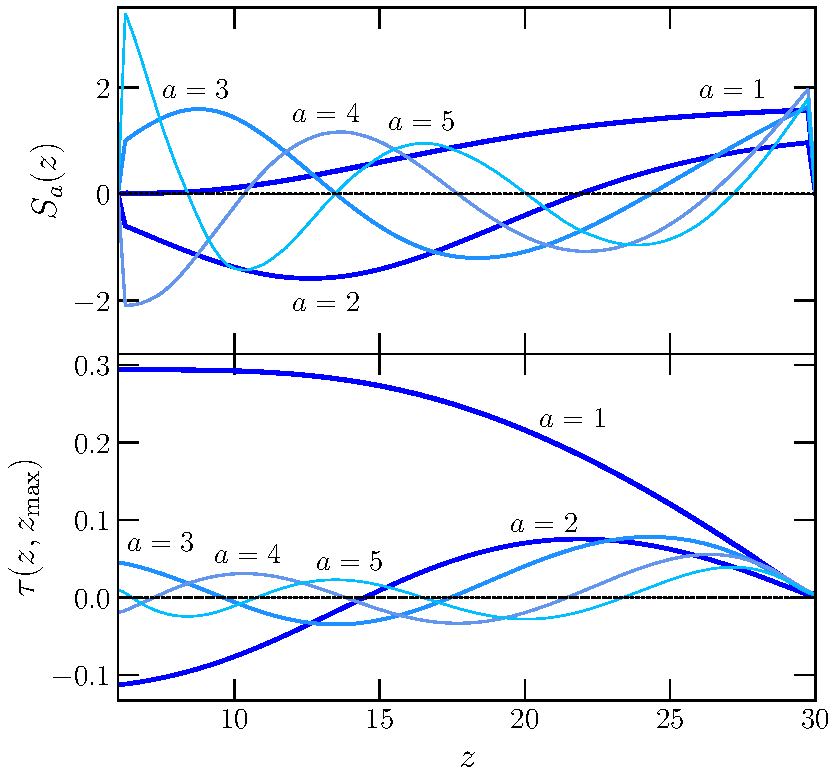
\includegraphics[width=0.48\textwidth]{paper/plots/pl18_plot_pub_xe_basis_tau_basis_zmax30_heinrich.pdf}
          \caption{\textit{Top}: Rank-ordered CMB reionization principal components $S_a$ for $a = 1..5$ for $\zmax = 30$. We assume fully ionized Universe at $z < 6$. \textit{Bottom}: The cumulative optical depth resulting from a unit amplitude PC. \ch{plot done}} 
          \label{fig:xe}
\end{figure}
 
\subsection{Reionization Principal Components}
\label{sec:PC}
We begin by parametrizing $x_e(z)$, the ionization fraction relative to the fully ionized hydrogen at redshift $z$, into its principal components $S_{a}(z)$ with respect to the CMB $E$-mode polarization:
%
\begin{equation}
x_e(z)=\xef(z)+\sum_{a}m_{a}S_{a}(z),
\label{eq:mmutoxe}
\end{equation}
%
where $m_a$ are the PC amplitudes and $\xef(z)$ is the fiducial model. We obtain the PC basis functions $S_{a}(z)$ as eigenfunctions of the Fisher information matrix for $x_e(z)$ in a given range $z_{\rm min}<z<z_{\rm max}$ from cosmic variance limited $C_\ell^{EE}$ measurements 
%
\beq
F_{ij} = \sum_l \frac{2 l+1}{2} \frac{\partial \ln C_l^{EE}}{\partial x_e(z_i)}\frac{\partial \ln C_l^{EE}}{\partial x_e(z_j)} = \sum_a \frac{ S_a(z_i) S_a(z_j)}{\sigma_a^2},
\eeq
%
where we have discretized the redshift space with $\delta z= 0.25$, and where $\sigma_a^2$ are the variances of the PCs.
The Fisher matrix is computed at a fiducial model which we take to be $x_e^{\rm fid}(z)=0.15$ in the parameterized range.
 Note that following Ref.~\cite{Heinrich:2018btc}, we have updated the PCs to be computed with Planck 2015 rather than WMAP best-fit 5 remaining $\Lambda$CDM parameters, which results in minor differences between the PC functions used in Ref.~\cite{Heinrich:2016ojb} and here. 


We then rank-ordered the PCs from low to high variance, so that for the range $z_{\rm min} = 6$ (to be consistent with Ly$\alpha$ forest constraints, e.g.~\cite{Becker:2015lua}) and $z_{\rm max} = 30$, only the first 5 components are needed to describe all the information on $x_e$ carried by $C_\ell^{EE}$ to cosmic variance limit. In the work that follows, we therefore truncate the sum at $a = 1 .. n_{\rm{PC}}$, where $n_{\rm{PC}} = 5$ for $z_{\rm max} = 30$ for the fiducial analysis.\footnote{We also test the robustness of our fiducial analysis in \S XX by  taking 
 for $z_{\rm max} = 50$ where $n_{\rm{PC}} = 7$ is required at the cosmic variance limit.}   
 
 
 
 
 In Fig.~\ref{fig:xe}
 %
 \footnote{There are very small differences between the PCs here and those shown in Ref.~\cite{Heinrich:2016ojb}, which can be attributed to a chance in the best-fit cosmology (WMAP to Planck 2015) when constructing the PCs.}
 %
 (top), we show the corresponding fiducial basis functions $S_a(z)$.  
Notice that the series resembles a Fourier decomposition of $x_e(z)$ rank ordered from low to high frequency.
This is because high frequency variations in $x_e$ leave little observable imprint in $C_l^{EE}$.  
As a consequence  the $n_{\rm PC}$ PCs are a complete representation of the \textit{observable impact} of $x_e(z)$ on the $C_\ell^{EE}$, rather than the ionization history itself. In other words, 
given any $x_e^{\rm true}(z)$, we can project it onto the $n_{\rm PC}$ PC basis through
\begin{equation}
m_{a}=
  \int _{\zmin}^{\zmax} dz\, \frac{S_{a}(z) [x_e^{\rm true}(z)-\xef(z)]}{\zmax-\zmin},
\label{eq:xetommu}
\end{equation}
%
where the reconstructed $x_e(z)$ through Eq.~(\ref{eq:mmutoxe}) with truncated PCs will not reproduce the true ionization history $x_e(z) \neq x_e^{\rm true}(z)$, but rather it is the observed $C_\ell^{EE}$ that is reproduced to cosmic variance precision. We reiterate therefore, that the PC analysis is not a tool for reconstructing the ionization history from observations, but rather a forward-modeling tool which, by reducing the dimensionality of the model space to $n_{\rm PC}$, allows us to constrain all possible ionization histories between $z_{\rm min}<z<z_{\rm max}$ in a single analysis.
For the Planck data set, most of the information on the ionization history comes from contraints on the first two modes which probe the amount of low vs.\ high redshift optical depth.   However all 5 PCs for $z_{\rm max}=30$ carry some constraint, with the higher modes controlling finer variations in redshift.

We follow Ref.~\cite{Heinrich:2018btc} to compute the CMB power spectra with PCs using a modified version of CAMB\footnote{CAMB: \url{http://camb.info}}~\cite{Lewis:1999bs, Howlett:2012mh}. 
For $z<6$, we follow CAMB and assume fully ionized hydrogen and singly ionized helium and for $z\leq 3.5$~\cite{Becker:2010cu}, doubly ionized helium~\cite{Becker:2010cu} with a transition width $\Delta z = 0.5$ (see also \S \ref{sec:example1}).


We obtain posterior constraints on the PC parameters $m_a$ from Markov Chain Monte Carlo sampling using COSMOMC\footnote{COSMOMC: \url{http://cosmologist.info/cosmomc}} of the relevant Planck likelihood discussed in \S \ref{sec:results} in an otherwise fiducial $\Lambda$CDM cosmology with the standard 5 parameters: the baryon density $\Omega_b h^2$, cold dark matter density 
$\Omega_c h^2$, effective angular sound horizon $\theta_{\rm MC}$, scalar power spectrum log amplitude $\ln (10^{10} A_s)$ and
its tilt $n_s$.  We take flat uninformative
priors in $m_a$ but discuss additional priors imposed by
removing demonstrably  unphysical ionization histories in \S \ref{sec:cumulative}.



%
%
%
%

\subsection{Effective PC Likelihood}
\label{sec:KDE}
The completeness property of the PCs enables us to turn PC chains obtained from a MCMC run into an effective likelihood that can be used to test any reionization model with the CMB without a cumbersome reanalysis at the level of power spectra data. In the following, we briefly recap the kernel density estimate (KDE) technique used to build this likelihood and refer the readers to Ref.~\cite{Heinrich:2016ojb} for more details.
The PC chains are composed of $N_{\rm sample}$ samples of discrete values of $\mathbf{m}_i = \{m_1, \ldots, m_5\}$ along with multiplicities $w_i$ for $i = 1$...$N_{\rm sample}$. Given any physical ionization history $x_e(z)$, we first obtain its PC representation $\mathbf{m}$ using Eq.~(\ref{eq:xetommu}). Since $\mathbf{m}$ can take any continuous value, we approximate its effective likelihood with a kernel density estimate
\beq
{\cal L}_{\rm PC}\left({\rm data}|\mathbf{m} \right)  = \sum_{i = 1}^{N_{\rm sample}} w_i K_f(\mathbf{m}-\mathbf{m}_i),
\eeq
where the overall normalization is arbitrary, and where we have chosen the smoothing kernel $K_f$ to be a  multivariate Gaussian with mean zero and covariance $f\mathbf{C}$, where $\mathbf{C}$ is the $N_{\rm PC} \times N_{\rm PC}$ covariance matrix estimated from the PC chains (see Table~\ref{tab:PC_stats}) and $f$ is a fraction smaller than 1.
For a Gaussian posterior, increasing the covariance by $1+f$ corresponds to increasing the standard deviation by approximately $1+f/2$. To minimize the amount of smoothing needed while still maintaining good accuracy in the tail of the distribution for any physical models, we oversample the PC distributions by running the PC chains far beyond convergence for about $N_{\sample} \approx 1.1 \times 10^{6}$ chain samples. 
% 1.06 cut w/ physicality prior
% 1.072 no cut
For this $N_{\sample}$, a fraction of $f = 0.14$ should be sufficient.
%Note also that we employ PC chains without the physicality priors allowing the smoothing kernel to cross over these priors. 
Evaluating the posterior distribution of model parameters $\bf p$ using the effective likelihood
\begin{equation}
P({\bf p}| {\rm data}) \propto {\cal L}_{\rm PC}\left[ {\rm data}|\mathbf{m}(\bf p) \right] P(\bf p).
\end{equation}

This approach obviates the need to implement specific reionization models into CAMB and conduct separate COSMOMC sampling for each, thereby significantly reducing both human and computational effort.
For comparison, an even simpler effective likelihood is the Gaussian approximation of the $m_a$ posterior using the PC mean $\bar{\bf m}$ and covariance $\bf C$
%
\begin{equation}
 {\cal L}_{\rm gauss}\left({\rm data}|\mathbf{m} \right) = \frac{ e^{-\frac{1}{2} ({\bf m}-\bar{\bf m})^T {\bf C}^{-1} ({\bf m}-\bar{\bf m}) } }{\sqrt{(2\pi)^{N_{\rm PC}} | \mathbf{C}| }}.
 \label{eq:gaussian}
 \end{equation}
%
In section~\ref{sec:effective_likelihood} we test the effective KDE and Gaussian approaches against a direct implementation
for two example models: the standard steplike model and a two-step model allowing for high-redshift ionization.


%
%
%
%We will compare its performance to the KDE likelihood for the Planck 2018 data in the two examples of section~\ref{sec:effective_likelihood} as well.
 
\subsection{Cumulative Optical Depth}
\label{sec:cumulative}

Although reionization PCs are mainly a tool for model testing using complete information from CMB polarization, as they do not reconstruct $x_e(z)$ itself, in particular the its rapidly  aspects, they do provide model-independent constraints on redshift integrated quantities such as  the cumulative Thomson optical depth
\begin{align}
\tau(z,z_{\rm max}) & = n_{\rm H}(0) \sigma_T \int_z^{z_{\rm max}} dz \frac{x_e(z) (1+z)^{2} }{H(z)}.
\end{align}
where $n_{\rm H}(0)$ is the hydrogen number density at $z=0$, $\sigma_T$ is the Thomson scattering cross-section and $H(z)$ is the Hubble parameter.   \wh{Given the tight constraints on cosmological parameters in the $\Lambda$CDM model, this quantity is well approximated by
\begin{align}
\tau_{\rm PC}(z,z_{\rm max})& = \sum_{a=1}^5 m_a \tau_a(z,z_{\rm max}) + \tau_{\rm fid}(z,z_{\rm max}),
\label{eq:cumtauPC}
\end{align}
where
\begin{align}
    \tau_a(z,z_{\rm max}) &= 
    n_{\rm H}^{\rm fid}(0) \sigma_T \int_z^{z_{\rm max}} dz \frac{S_a(z) (1+z)^{2} }{H_{\rm fid}(z)}, \nonumber\\
    \tau_{\rm fid}(z,z_{\rm max}) &= 
    n_{\rm H}^{\rm fid}(0) \sigma_T \int_z^{z_{\rm max}} dz \frac{x_e^{\rm fid}(z) (1+z)^{2} }{H_{\rm fid}(z)},
\end{equation}
 where ``fid" refers to evaluation in the fiducial cosmology.   When we omit the redshift arguments, we implicitly mean the total range, e.g. $\tau_{\rm PC}=\tau_{\rm PC}(0,z_{\rm max})$. }
 
 \wh{
 In Fig.~\ref{fig:xe}, we display $\tau_a(z,z_{\rm max})$.
 Notice that positive values of the first component $m_1$ mainly provides the optical depth that is accumulated at high redshift whereas {\it negative} values of $m_2$ provides the same for low redshift.    Since these two are the best measured components, the CMB mainly determines the amount of low vs.~high redshift ionization.
The underlying reason is that in $C_l^{EE}$ the higher the redshift, the
larger the relative contribution at higher $l$ due to the size of the horizon when the photons scattered.  For the less well measured PCs with $a>2$, the contributions to the total optical depth rapidly diminish and represent finer distinctions in redshift for the cumulative optical depth.}

\wh{
In the usual approach to constraining reionization in $\Lambda$CDM, one places an implicit prior on the shape of the cumulative optical depth by choosing a model like a near step function reionization and then extracts a single constraint on the total optical depth.}
%For example, the standard steplike model adopted in CAMB uses a width=0.48 function to parameterize the hydrogen and singly ionized helium reionization
% \begin{equation}
%x_e^{\rm true}(z) = \frac{1+f_{\rm He}}{2}\left\{  1+ \width=0.48\left[ \frac{y(z_*)-y(z)}{\Delta y} \right] \right\},
% \label{eqn:tanh}
% \end{equation}
% where $y(z)=(1+z)^{3/2}$, $\Delta y=(3/2)(1+z)^{1/2}\Delta z$, and $\Delta z = 0.5$,
% excludes finite ionization above its transition redshift by definition.
The PCs on the other hand, allow for arbitrary values of $x_e(z)$ when no range-bound prior constraints on the mode amplitudes $m_a$ are imposed. The one subtlety when placing constraints on the cumulative optical depth is that the analysis also allows
unphysical ionization fractions where $0 \le x_e \le x_e^{\rm max}$  is not satisfied.
Therefore, when determining cumulative optical depth constraints as opposed to using reionization PCs as a tool for testing models,
 we do impose a  prior
 by truncating the posteriors of $m_a$
 {\it after} obtaining them from Markov Chain Monte Carlo sampling, following Ref.~\cite{Mortonson:2008rx}
%
\begin{equation}
\sum_{a=1}^5 m_a^2 \le (x_e^{\rm max}-x_e^{\rm fid})^2,
\label{eq:prior_sum}
\end{equation}
where $x_e^{\rm fid}=0.15$ and $m_a^{-} \le m_a \le m_a^{+}$ with
\begin{equation}
m_a^{\pm} = \int_{z_{\rm min}}^{z_{\rm max} } dz \frac{S_a(z)[x_e^{\rm max} -2 x_e^{\rm fid}(z)]
\pm x_e^{\rm max} | S_a(z)|}{2(z_{\rm max}-z_{\rm min})}.
\label{eq:individualprior}
\end{equation}
\wh{Here we take $x_e^{\rm max} = 1+ n_{\rm He}/n_{\rm H}$ to account for the contribution of singly ionized helium.}
In practice the prior on the sum of squares in Eq.~(\ref{eq:prior_sum}) is strictly weaker than the individual priors in Eq.~(\ref{eq:individualprior}) for
% I think it can't depend on the data but does depend on the truncation
%the Planck 2018 data \wh{and
our fiducial analysis.  Henceforth we refer to Eq.~(\ref{eq:individualprior}) as the physicality prior.

%
Note that the original $0\le x_e \le x_e^{\rm max}$ condition cannot be strictly enforced here because we do not keep all but the first $n_{\rm PC}$ PCs, so these priors in $m_a$ are necessary but not sufficient conditions for a physical ionization history.  
In other words, no physical model is excluded by these priors but some unphysical models are included.  In \S \ref{sec:note_on_priors} we further explore the role of these and other choices of PC priors, and in \S\ref{sec:effective_likelihood} we test PC constraints against direct constraints for two example models.  



\section{Planck 2018 PC Results}
\label{sec:results}
We now present the complete reionization constraints obtained from the Planck 2018 likelihoods using the principal components.
\subsection{Constraints on Principal Components}
We use the official Planck likelihoods [add citation] \texttt{plik\_lite} for the high-$\ell$ $TT$, $TE$ and $EE$ as well as \texttt{lowl} for the low-$\ell$ $TT$ throughout this paper. We have tested that our results do not change if in lieu of \texttt{plik\_lite} we used the full \texttt{plik\_full} likelihood in which the foreground parameters have not been marginalized over. For the low-$\ell$ $EE$ likelihood, we use the third-party released \texttt{srollv2} likelihood [add citation] in our official PC results and the effective likelihood code. In comparison with the official Planck-released \texttt{simall\_EE} likelihood, the \texttt{srollv2} likelihood improves foreground cleaning, 
which enables stronger reionization constraints, especially for the low multipole moments that are important for the low redshift constraints.

% can add a comment about impact 
%d a factor of XX improvement in $\tau$ just in the steplike model [cite].


\begin{figure*}
%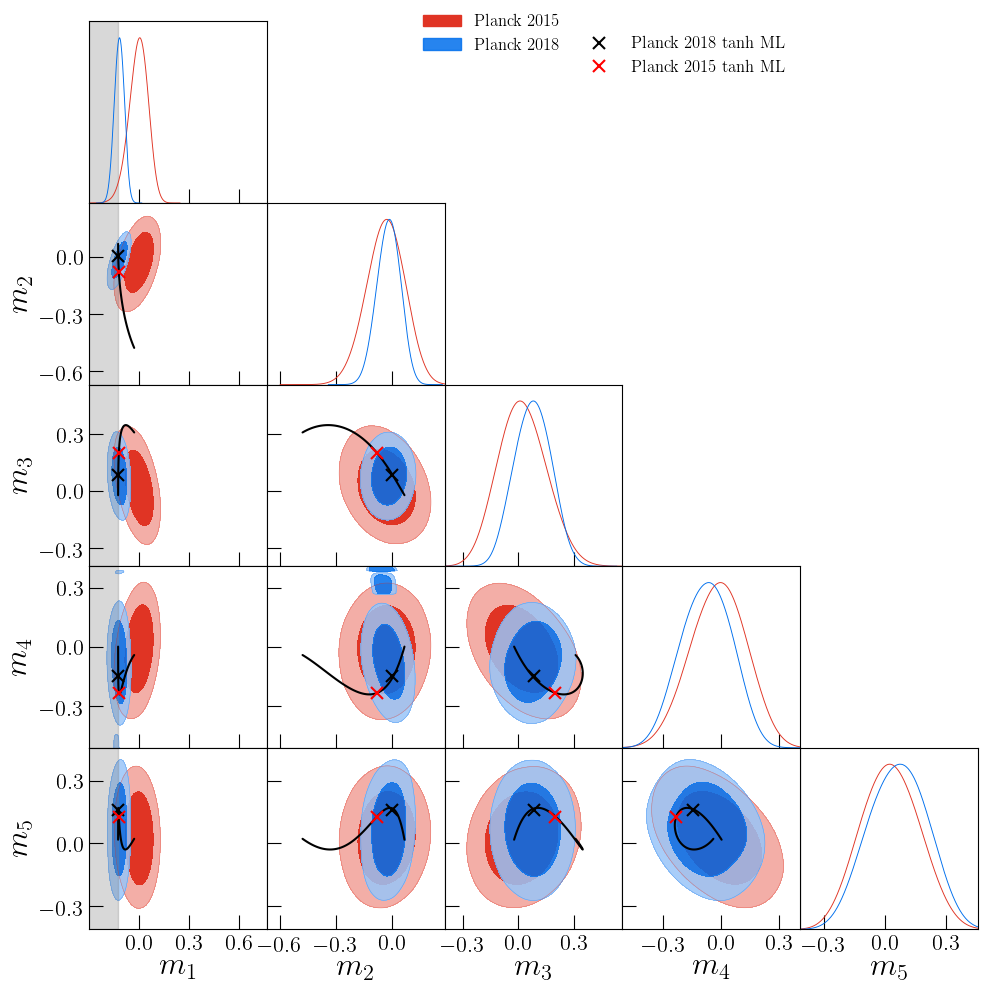
\includegraphics[width=0.7\textwidth]{plots/plot_mj_triangle_t18_r12_t19_t20_vs_pl18_pc_zmax30_pliklite_srollv2_1015_wTauTrajectory_pl15_wTanhML.png}
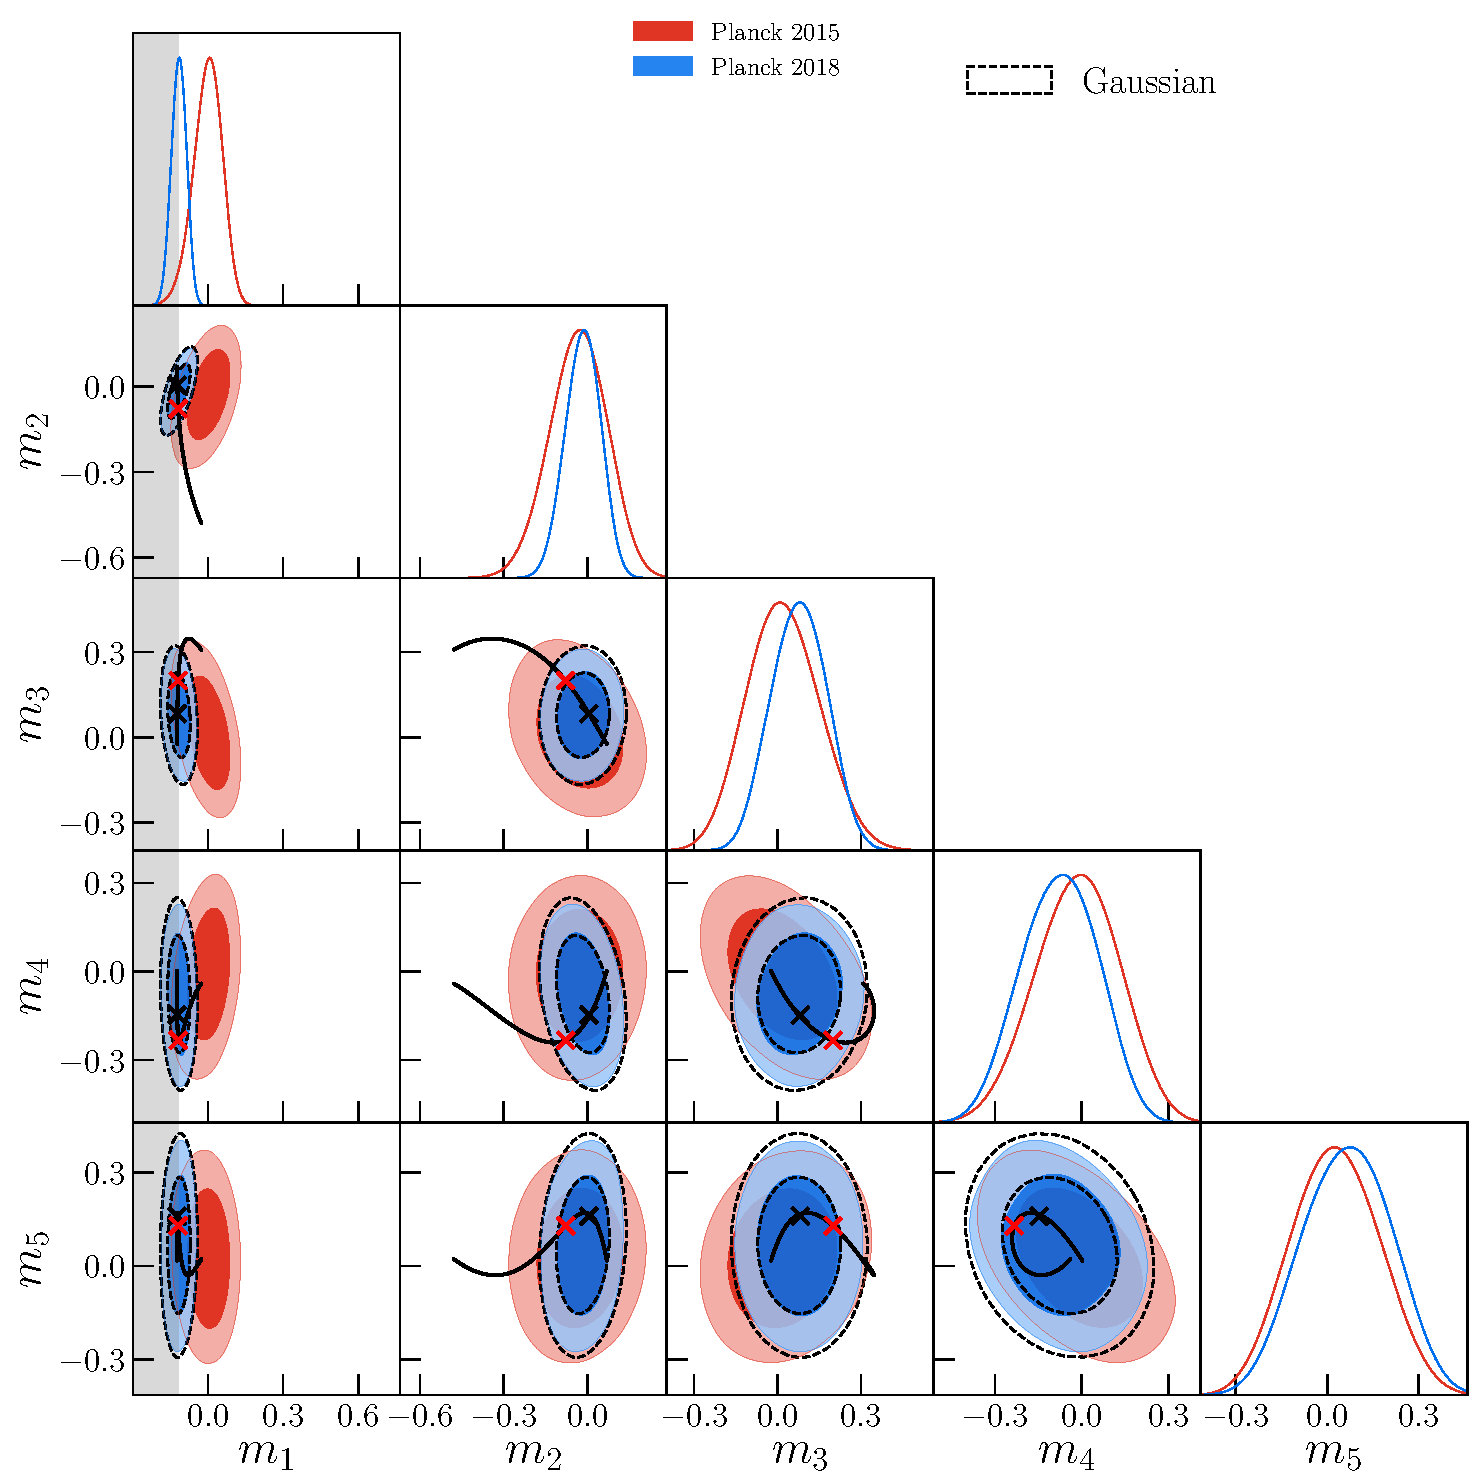
\includegraphics[width=0.8\textwidth]{paper/plots/plot_mj_triangle_t18_r12_t19_t20_vs_pl18_pc_zmax30_pliklite_srollv2_1015_wTauTrajectory_pl15_wTanhML_wGaussEllipse.pdf}

\caption{Constraints from Planck data on the amplitudes of the five reionization principal components that describe all physical ionization models up to $z_{\rm max} = 30$. We show in red the Planck 2015 and the improved Planck 2018 contours in blue which uses the low-$\ell$ $EE$ likelihood \texttt{srollv2}. The 1D posterior distributions are shown on the diagonal and the 2D 68\% and 95\% C.L. regions in the $m_a-m_b$ planes in the lower triangle. The physicality priors on the ionization history used in this work are delineated by the box boundaries and the unshaded region for $m_1$. The black solid line indicates the tanh models with varying $\tau$. The red and black crosses indicate the best-fit tanh models from Planck 2015 and 2018 respectively. Note that the best-fit tanh model has moved to a lower $\tau$ in Planck 2018, and in particular, is now within the 68\% C.L. contours of the constraints. \ch{plot done}
}
\label{fig:plot_mjs_2018_vs_2015}
\end{figure*}
%
%
In Fig.~\ref{fig:plot_mjs_2018_vs_2015}, we show the 1D posterior and 2D 68\% and 95\% confidence level contours for the 5 PC amplitudes that describe ionization models up to $\zmax=30$
%
\footnote{We The Planck 2015 best-fit is derived from a chain best-fit model as taken from Ref.~\cite{Heinrich:2016ojb}, whereas for the Plnack 2018 point in this paper we used a minimizer to find the best-fit; there are also slight model differences, where in Planck 2018 we used a tanh width of $dz = 0.015(1+z)$ instead of $dz = 0.5$ for the Planck 2015 best-fit. Using $dz = 0.5$ for Planck 2018 moves the cross negligible on this plot.}.
%
The shaded region in the $m_1-m_2$ plane represents the parameter region that would be excluded by an additional 
physicality prior from Eq.~(\ref{eq:individualprior}), whereas for the other cases the box itself represents this prior. Results using the Planck 2018 data are shown in blue. While all five PC amplitudes are  constrained by Planck, the first two are particularly well-constrained. Contrary to the Planck 2015 results of Ref.~\cite{Heinrich:2016ojb} shown in red, the 2018 data prefers a much smaller amplitude for the first PC, leading to a reduced optical depth.  \wh{This preference also increases the impact of placing a physicality prior at low values of $m_1$.
We show a zoomed version of the $m_1-m_2$ plane in Fig.~\ref{fig:plot_m1m2_2015_vs_2018}.
In this excluded region, the optical depth of models are dominated by the low redshift end, but due to the fixed ionization at $z>z_{\rm min}=6$, the desired total optical depth cannot be achieved without an unphysical ionization elsewhere.} \ch{[Not sure if we should say ``In this excluded region" referring to the entire gray band, or specify overlap with data constraints where $m_2 < 0$ mostly?]}

In Fig.~\ref{fig:plot_m1m2_2015_vs_2018}, we also show
the Planck 2018 constraints using the older \texttt{simall\_EE} likelihood.  The improvement 
from switching to the \texttt{srollv2} likelihood mainly strengthens the upper bound in the best constrained direction in the $m_1-m_2$ plane which shifts constraints toward higher total optical depth.

\wh{possibly point to a figure below with $\tau_{12}$ in}

%\wh{possibly move the discussion of trajectories into the model section}
%The trajectories shown in black lines are the steplike models of instantaneous reionization allowed by the Planck 2015 data with the arrow pointing in the direction of increasing optical depth. Clearly, these steplikes models are only a part of the allowed physical model space. By construction, they miss any high-redshift ionization component by assuming neglibile ionization levels before the transition redshift $z_{\rm re}$. 

\begin{figure}
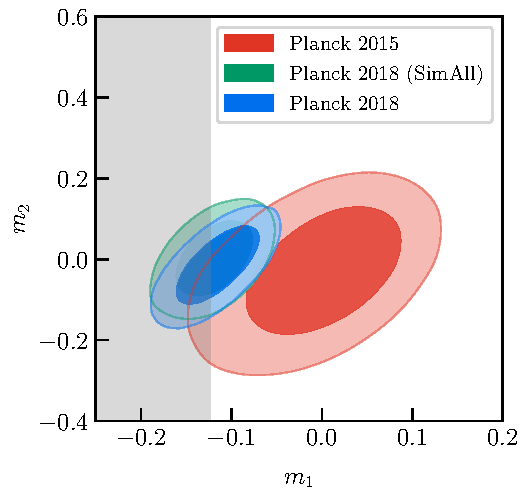
\includegraphics[width=0.40\textwidth]{plots/plot_m1_m2_t18_r12_t19_t20_vs_pl18_pc_zmax30_pliklite_0930_vs_pl18_pc_zmax30_pliklite_srollv2_1015.pdf}
\caption{A zoomed-in of Fig.~\ref{fig:plot_mjs_2018_vs_2015} on the best constrained $m_1-m_2$ PC plane. We compare the Planck 2015 (gray) to the Planck 2018 constraints using two different low-$\ell$ $EE$ likelihoods: the \texttt{simall\_EE} likelihood (red) and the \texttt{srollv2} likelihood (blue). The \texttt{srollv2} likelihood used better foreground removal and is what we use as our fiducial results throughout this paper. 
}
\label{fig:plot_m1m2_2015_vs_2018}
\end{figure}

\begin{table}[b]
\centering
\caption{PC chain means $\bar m_a$, standard deviations $\sigma(m_a)$, and correlation matrix $R_{ab}$. \ch{transpose this table and add a row for taumj, and quote taufid in the caption}}
\label{tab:PC_stats}
\begin{tabular}{|r | r r@{\hskip 0.06in}|r r r r r|}
\hline
		
			  &  \multicolumn{1}{c}{$\bar m_a$} & \multicolumn{1}{c}{$\sigma(m_a)$}	 & \multicolumn{1}{|c}{$m_1$} & \multicolumn{1}{c}{$m_2$} & \multicolumn{1}{c}{$m_3$} & \multicolumn{1}{c}{$m_4$} & \multicolumn{1}{c|}{$m_5$} 
		\\ \hline
		

$m_1$ & $-$0.116 & 0.030 & 1.000 & 0.657 & $-$0.208 & $-$0.094 & 0.067 \\
$m_2$ & $-$0.016 & 0.063 & 0.657 & 1.000 & 0.048 & $-$0.273 & 0.142 \\
$m_3$ & $$0.078 & 0.098 & $-$0.208 & 0.048 & 1.000 & 0.064 & $-$ \\
$m_4$ & $-$0.077 & 0.131 & $-$0.094 & $-$0.273 & 0.064 & 1.000 & $-$0.195 \\
$m_5$ & 0.066 & 0.145 & 0.067 & 0.142 & $-$0.018 & $-$0.195 & 1.000 \\

\hline
\end{tabular}
\end{table}

\begin{table}[b]
\centering
\caption{$\tau_a$}
\label{tab:PC_stats}
%\begin{tabular}{|r | r r r r r r|}
\begin{tabular}{|c | c | c | c | c | c|}
\hline
$\tau_{\rm fid}$ & $\tau_1$  & $\tau_2$ & $\tau_3$ & $\tau_4$ & $\tau_5$ \\ \hline
0.08626 & 0.29403 & $-$0.11227 & 0.04506 & $-$0.01898 & 0.00960 \\
\hline
\end{tabular}
\end{table}
% all digits without flipping m3, m4:
%tau_fid 0.08625526676478058
%taumj [ 0.29403315 -0.11227135 -0.04505736  0.0189787   0.00960184
\begin{table}[b]
\centering
\caption{Planck 2015 results (with Mortonson PCs) [Will not be in the paper, just for us to compare] }
\label{tab:PC_stats}
\begin{tabular}{|r | r r@{\hskip 0.06in}|r r r r r|}
\hline
		
			  &  \multicolumn{1}{c}{$\bar m_a$} & \multicolumn{1}{c}{$\sigma(m_a)$}	 & \multicolumn{1}{|c}{$m_1$} & \multicolumn{1}{c}{$m_2$} & \multicolumn{1}{c}{$m_3$} & \multicolumn{1}{c}{$m_4$} & \multicolumn{1}{c|}{$m_5$} 
		\\ \hline

$m_1$ 
	& 0.002 & 0.053 & 1.000 & 0.450 & $-$0.432 & 0.273 & $-$0.073 \\ 
$m_2$ 
	& $-$0.030 &  0.101 & 0.450 & 1.000 & $-$0.262 & 0.055 & 0.072 \\ 
$m_3$ 
	& 0.019 &  0.128 & $-$0.432 & $-$0.262 &1.000 & $-$0.417 & 0.155 \\
$m_4$  
	& $-$0.012 & 0.143 &  0.273 & 0.055 & $-$0.417 & 1.000 & $-$0.428 \\ 
$m_5$ 
	& 0.026 & 0.143 & $-$0.073 & 0.072 & 0.155 & $-$0.428 & 1.000\\ 
\hline
\end{tabular}
\end{table}


We show a zoomed version of the $m_1-m_2$ plane in Fig.~\ref{fig:plot_m1m2_2015_vs_2018}, where we show beyond the physicality prior with the shaded area. [Discuss how the ellipse moved in the direction of lower tanh by going to lower m1.] 


In Fig.~\ref{fig:plot_mjs_2018_vs_2015}, we also show the constraints assuming a Gaussian posterior in $m_a$ using the PC chain covariance and means listed in Table~\ref{tab:PC_stats}.  The visual agreement with the full posteriors is remarkably good, especially in the well constrained components.  This suggests that the simple Gaussian  likelihood of Eq.~(\ref{eq:gaussian}) may suffice for rough constraints on models.    However we shall see that a quantitative comparison shows that there is enough skewness in the posteriors that the KDE likelihood 
still performs noticeably better.  \wh{revisit this 
statement once we firm up the comparison, e.g. what is noticeably better, means, 95\% confidence intervals, far tails?} \ch{yup, will do.}

% This Gaussian approximation agrees well with the actual PC constraints, unlike in the Planck 2015 data where some differences were still visible on top of good agreement. The Gaussian likelihood is even faster than the kernel density estimate. As shall see in the next section for two explicit examples, the Gaussian likelihood shows generally good agreement with the full KDE result, but is unable to capture, as expected given its symmetric nature, any skewness in the PC distribution that may affect parameter constraints.

%In Fig.~\ref{fig:plot_m1m2_lowE_vs_srollv2} we also compare the Planck 2018 results with two different low-$\ell$ $EE$ likelihoods: \texttt{simall\_EE} and \texttt{srollv2}. The \texttt{srollv2} contours are shrunk nearly directly along the lines of constant optical depth $\tau$ ($\tau_{12} = \tau_1 m_1 + \tau_2 m_2$) [wanna show this]? \wh{we might make this point in the context of Marius - that $\tau$ is mainly a linear function of $m_1$, $m_2$, and hence flat priors in $m's$ are locally flat in $\tau$}.

\section{Model Testing with PCs}
\label{sec:effective_likelihood}

We now turn to constraining reionization models with PCs using the
effective likelihood approach described in~\refsec{KDE}.  The benefit of this approach is that
complete constraints on any model of the ionization history  between $6 \leq z \leq \zmax$ can now be obtained without reanalyzing the Planck data. 
This effective likelihood code is available on GitHub at \url{} [give URL]. The initial release corresponds to our fiducial constraints derived from the Planck 2018 $\texttt{plik\_lite\_TTTTTE} + \texttt{lowl} + \texttt{srollv2}$ likelihood combination with $\zmax = 30$. 

To use this approach, one simply specifies the functional form for $x_e(z)$ in the code, which then is converted to the PC parameters $m_a$ for the effective likelihood evaluation assuming a \ch{fiducial} $\Lambda$CDM cosmology.   
To obtain reionization model parameter posteriors, one samples this likelihood with any desired priors.   
We have also provided an MCMC sampler for models of high dimension (currently in CosmoMC). Note that the model parameters or priors must be arranged to explicitly satisfy 
full ionization below $z=6$. To avoid over-smoothing parameter posteriors while maintaining accuracy during the KDE operation, we suggest using the default value of $f = 0.14$.

Next we demonstrate the use and the successful recovery of parameter posteriors using the effective likelihood code by comparing them to a direct MCMC analysis for two examples: 1) The tanh model, which is the standard approach used in CAMB; 2) a two-step toy model which has one additional parameter modeling a high-$z$ ionization plateau before the transition to full ionization in the canonical tanh model.

\subsection{Example 1: tanh model}
\label{sec:example1}

\begin{figure}
\includegraphics[width=0.48\textwidth]
%normalized by area
%{results/tau_posterior_comparisons/pl18_tau_posterior_tanh_vs_tanh_kde_vs_tanh_gaussian_dz_auto_zre_prior_6p1_normalized_by_area.pdf}
%normalized by max
{results/tau_posterior_comparisons/pl18_tau_posterior_tanh_vs_tanh_kde_vs_tanh_gaussian_dz_auto_zre_prior_6p1_normalized_by_max.pdf}
\caption{Comparison of the total optical depth posterior for the tanh model in \refsec{example1} between the full Planck likelihoods (solid), our effective likelihood in the kernel density estimate mode with $f = 0.14$ (dotted), and in the Gaussian approximation mode (dashed) \ch{tune plot and line styles}. The KDE mode agree well with the full results, while giving a slightly broader posterior because the kernel density estimate in the PC space introduces smoothing at roughly $\sim$7\% level in the parameter posterior corresponding to $f = 0.14$. The Gaussian likelihood works well too, with no extra broadening of the posterior, but a negligible shift in the mean ($\sim XX\%$ of the error in $\tau$). This posterior is symmetric and does not capture the small skewness found in the full and KDE chains. \ch{might need to rephrase. \ch{This plot is done. Changed convention to normalization by max; to restore figure normalized by area, see comments in latex.}}
}
\label{fig:tanh}

\end{figure}
\begin{figure}[ht]
\includegraphics[width=0.48\textwidth]
%normalized by area
%{results/tau_posterior_comparisons/pl18_tau_posterior_tanh_vs_tanh_highz_vs_pc_dz_auto_zre_prior_6p1_normalized_by_area.pdf}
%normalized by max
{results/tau_posterior_comparisons/pl18_tau_posterior_tanh_vs_tanh_highz_vs_pc_dz_auto_zre_prior_6p1_normalized_by_max.pdf}
\caption{\ch{P(tau) PC (with and without prior) vs tanh vs tanh highz (normalized by max)}}
%double check plot, upper and lower limits seem to cross?
\label{fig:plot_tau_posterior_PC_vs_tanh_vs_tanh_highz}
\end{figure}

\begin{figure}[ht]
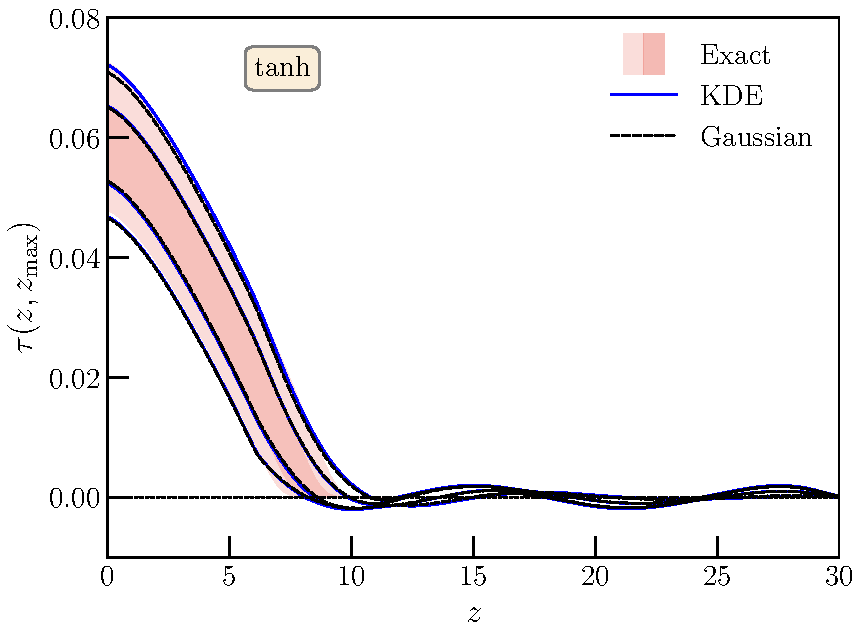
\includegraphics[width=0.48\textwidth]{paper/plots/pl18_taugtz_tanh_direct_vs_kde_vs_gaussian.pdf}
\caption{Comparison of the 68\% and 95\% C.L. constraints on the cumulative optical depth in the tanh model (described in \refsec{example1}) between the full Planck likelihoods (shaded bands), our effective likelihoods in the KDE mode (blue solid) and Gaussian mode (black dashed). The effective likelihoods results oscillate around zero at high-z because of the truncated representation of the models at 5 PCs (enough to represent any observable effects in the data). While the Gaussian approximation performs fairly well, the more complete KDE mode gives a slightly more accurate 95\% limits on the total optical depth. \ch{add numbers in caption: 95\% (0.039, 0.02), best-fit (0.05290344, 0.005859431)}}
%double check plot, upper and lower limits seem to cross?
\label{fig:plot_taugtz_PC_vs_tanh}
\end{figure}

The steplike model used as the standard approach in CAMB describes the hydrogen and singly ionized helium reionization as a tanh function:
%
 \begin{equation}
x_e(z) = \frac{1+f_{\rm He}}{2}\left\{  1+ \tanh\left[ \frac{y(z_{\rm re})-y(z)}{\Delta y} \right] \right\} + x_e^{\rm rec},
 \label{eqn:tanh_1D}
 \end{equation}
 %
 with $y(z)=(1+z)^{3/2}$, $\Delta y=(3/2)(1+z)^{1/2}\Delta z$. Instead of using $\Delta z = 0.5$ as in the standard setting by camb, we adopt a smaller width $\Delta z = 0.015(1+z)$ so as to better capture the required full ionization below $z=6$. Here $x_e^{\rm rec}$ is the ionization history from recombination only; the helium fraction
 \beq
 f_{\rm He} = \frac{n_{\rm He}}{n_{H}} = \frac{m_{\rm H}}{m_{\rm He}} \frac{Y_p}{1 - Y_p}, 
 \eeq
 is the ratio of the helium to hydrogen number density, where $Y_p$ is the helium mass fraction, chosen to be consistent with big bang nucleosynthesis for a given baryon density. In addition, the doubly ionized helium reionization is parameterized by an additional tanh function in redshift centered at $z_{\rm He} = 3.5$ with width $\Delta z = 0.5$.

The $\tanh$ model is parameterized by its total optical depth $\tau$ for which we take a flat prior 
with an additional constraint that $z_{\rm re}\ge 6.1$ so as to better satisfy the required $z_{\rm min}=6$ given $\Delta z$.
In Fig.~\ref{fig:plot_mjs_2018_vs_2015}, we show the trajectory that the $\tanh$ model takes in the PC space. Notice that this trajectory passes near the center of all constraints for Planck 2018 but only through the tails for some of the Planck 2015 constraints.  Correspondingly, whereas the $\tanh$ model was marginally disfavored with Planck 2015 data that is not the case with Planck 2018 data. 

In \reffig{tanh} we show the posterior distribution of $\tau$ for the effective likelihood results, in which the only sampled parameter is $\tau$ (all other cosmological parameters are fixed at the Planck best-fit model), vs the full likelihood results in which the five other $\Lambda$CDM parameters were also varied using the same priors for the $\tanh$ model.
%including $\tau$. 
%Because the PC method cannot accurately represent models that are not fully ionized below $z = 6$, we apply a prior $\zre < 6.1$ to both chains given the transition width of about $0.015(1+z) \approx 0.1$ at $z = 6$. 
The posteriors agree well; the effective likelihood gives a slightly broader posterior because the kernel density estimate in the PC space introduces smoothing. We expect the smoothing to be roughly at the $\sim$7\% level in the parameter posterior corresponding to a smoothing factor of $1+f = 1.14$ applied to the covariance of the PCs used for smoothing kernel during KDE. Indeed, the KDE result $\tau = 0.0588 \pm 0.0066$ has a negligibly lower mean ($0.05\sigma$) and a 6.5\% larger standard deviation (as expected) than the full likelihood result $\tau = 0.0591 \pm 0.0062$.

Instead of the effective likelihood, we can alternately use its Gaussian approximation shown in Eq.~(\ref{eq:gaussian}). The Gaussian likelihood is faster to evaluate as it does not require looping over the entire $\sim 10^6$ points in the PC chain. [add timing here]
%and amounts to one evaluation of the multi-variate Gaussian function per sample in the reionization model parameter space. 
We obtain for the tanh model $\tau = 0.0594 \pm 0.0063$. While it is a good approximation (the mean and standard deviation are similar to those from the full likelihood and the effective likelihood using KDE), we see in Fig.~\ref{fig:tanh} that the peak of the distribution for the Gaussian likelihood is offset from the other two. This is because the Gaussian likelihood is by definition symmetric in the PC space and so it cannot capture any skewness in the PC distribution. As a result the tanh $\tau$ constraints are mostly symmetric too, $\tau = 0.0594_{-0.0064}^{+0.0064}$ if we consider the 68\% lower and upper limits, whereas the full KDE result $\tau = 0.0588_{-0.0072}^{+0.0060}$ is able to capture the skewness in the distribution $\Delta \tau \sim 0.0012$, a level consistent with shifts in the peaks seen in Fig.~\ref{fig:tanh}.

\ch{[double check all these numbers again (some chains are longer now)]}.

[Make a point that dz = 0.5 for tanh may not be sufficient for experiments after Planck. This was for higher tau, so transition happens at higher redshift. Now tau is much lower.] 

[Note sure if it is related to this statement in Planck 2018 paper: ``The TANH result gives slightly higher optical  depth  than  the  others,  which  is  primarily driven  by  the  fixed  duration  of  reionization assumed.” Is this true? Then transition to the following point]


We also show in Fig.~\ref{fig:plot_taugtz_PC_vs_tanh} the cumulative optical depth obtained from directly integration the exact tanh model in the full likelihood chains vs that from the 5-PC representation of the tanh models in the effective likelihood chains. [describe more once plot is made]. From these constraints it is also clear that the tanh model does not allow for high redshift ionization by construction, while the PC chains sampling the entire space of physical models would still allow for some high-$z$ ionization in the Planck 2018 data, as we shall see later in in Section~\ref{sec:results}.

\subsection{Example 2: high-z model}
\label{sec:example2}

\wh{pick a consistent name for this model and use it for the section title, discussion, figure captions and labels - much of the discussion uses ``two step" which would be fine and may be better than high-z}

\begin{figure}
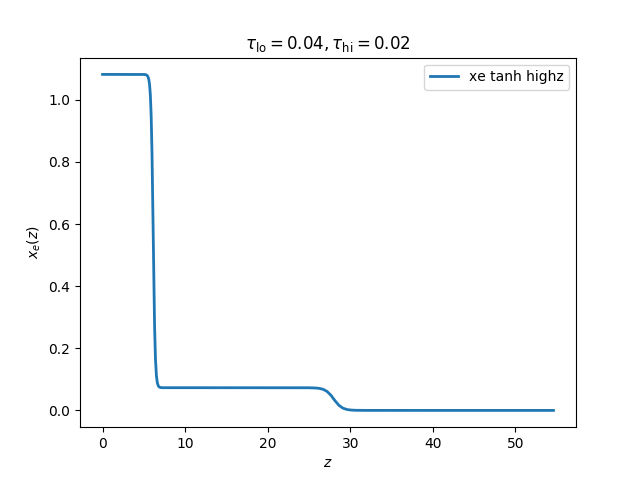
\includegraphics[width=0.48\textwidth]{results/cosmomc_kde/taulo_prior_test/plot_xez_taulo_0p04_tauhi_0p02.png}
\caption{Example ionization history $x_e(z)$ for the high-$z$ model of \refsec{example2}. In addition to a tanh transition at low-redshift as in \refsec{example1}, there is an additional ionization plateau at high redshifts with a fixed transition at $z_t = 28$ and $\Delta z = 1$. This is a toy model constructed for illustration purposes only. Here we show the best-fit model in the Planck 2018 data $(\taulo, \tauhi) = (XX, XX)$, as well as  a model at the 95\% C.L. $(\taulo, \tauhi) = (XX, XX)$ (see also Fig.~\ref{two_parameter_model_2}  \wh{place x's on the models plotted in that plot}). \ch{Include 2nd helium in the plot.}
}
\label{fig:two_step_model}
\end{figure}

%
%

\begin{figure}[t]
%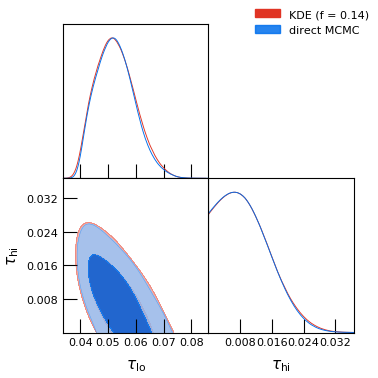
\includegraphics[width=0.47\textwidth]{results/cosmomc_kde/pl18_tanh_highz_test5_run1_vs_relike_tanh_highz_test8_run9_f0p14_taulo_prior_0p03_zre_prior_6p1_taulo_prior_0p0_tri.png}
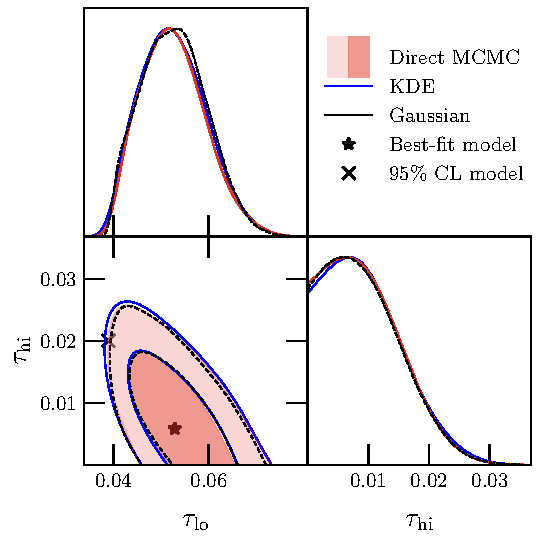
\includegraphics[width=0.48\textwidth]{paper/plots/pl18_tanh_highz_test5_run1_vs_relike_tanh_highz_test8_run9_f0p14_taulo_prior_0p03_zre_prior_6p1_taulo_prior_0p0_tri.pdf}
\caption{\ch{Need to fix this plot.}   Comparison of the marginalized posteriors and the 2D 68\% and 95\% C.L. contours for the two-step model  described in \refsec{example2} between different likelihoods: The full Planck likelihoods (shaded), the effective likelihoods in the KDE mode with f = 0.14 (blue solid) and in the Gaussian approximation mode (black dashed). The results agree well with each other. As in Fig.~\ref{fig:tanh}, both the KDE and Gaussian modes agree very well with the full likelihood results, with the KDE  contours being slightly broader as expected.
}
\label{fig:two_parameter_model_2D}
\end{figure}

\begin{figure}
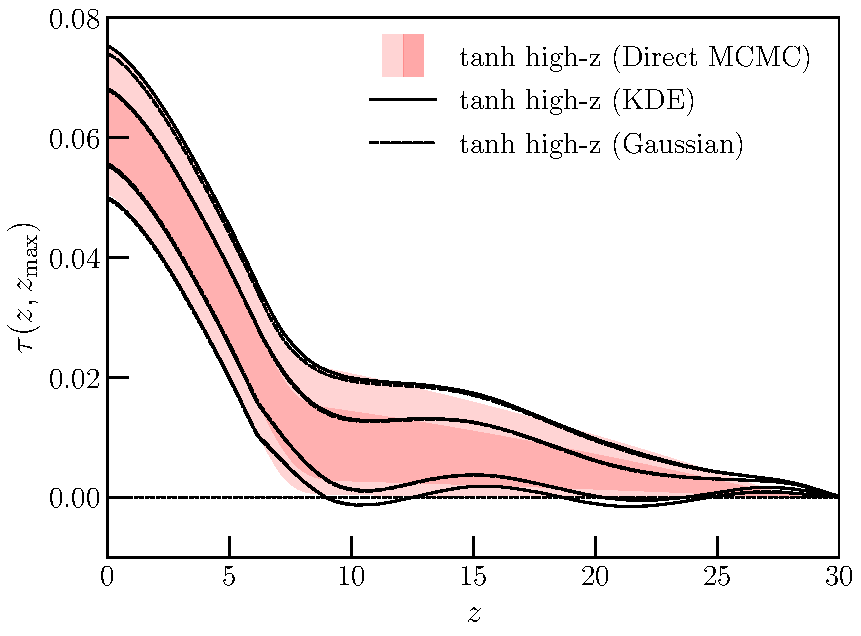
\includegraphics[width=0.48\textwidth]{plots/pl18_taugtz_tanh_highz_direct_vs_kde_vs_gaussian_dz_auto_zre_prior_6p1.pdf}
\caption{Comparison of the 68\% and 95\% C.L. constraints on the cumulative optical depth $\tau(z, \zmax)$ for the two-step model, which allows for high-redshift ionization up to $\zmax =30$. Note that a physical model with $\tau(15, \zmax) = 0.02$ is still allowed at the 95\% C.L. whereas it is ruled with the Planck official results using the FlexKnot method $\tau(15, \zmax) < 0.007$. Here again, the KDE and Gaussian likelihoods agree well with the full likelihoods, with better 95\% C.L. limits on the total optical depth. The truncation at 5 PCs causes wiggles at higher redshifts, but these cause negligible differences at most redshifts.
\ch{CH: plot is done}}
\label{fig:plot_taugtz_two_step_contours}
\end{figure}
 
 
The second example is a two-step model, where an additional step is used to give a high-$z$ ionization plateau: 
 \bea
x_e&(z)&\,= \frac{1+f_{\rm He} - \xemin}{2}\left\{  1+ \tanh\left[ \frac{y(z_{\rm re})-y(z)}{\Delta y} \right] \right\} \notag \\
&+& \frac{\xemin - x_e^{\rm rec}}{2}\left\{  1+ \tanh\left[ \frac{z_{\rm t}-z}{\Delta z_{2}} \right] \right\} + x_e^{\rm rec},
 \label{eqn:tanh_highz}
 \eea
where $y(z)=(1+z)^{3/2}$, $\Delta y=(3/2)(1+z)^{1/2}\Delta z_1$ where $\Delta z_1 = 0.015\, (1+z_{\rm re})$ just as in the first example for a sharper step.
We choose the second step at $z_{\rm t}=28$ with $\Delta z_2 = 1.0$, since the effective likelihood is limited to models with ionization below $\zmax=30$. 
In comparison to tanh, a single parameter $\xemin$ is added in this model to control the high-$z$ ionization plateau for $z_{\rm re} \lesssim z \lesssim z_t$. We would recover the standard tanh as $\xemin$ approaches the negligible recombination value $x_e^{\rm rec}$. We show an example
of this two-step model in Fig.~\ref{fig:two_step_model}.



In practice, we parameterize the model by $\taulo(\zre, \xemin)$ and $\tauhi(\zre, \xemin)$.  They are defined as in \refeq{cumtau} but with the boundaries $[0, z_{\rm split}]$ and $[\tau(z_{\rm split}, \infty]$ for $\taulo$ and $\tauhi$ respectively, where the split is chosen as $z_{\rm split} = \zre + \Delta z_2$ to be conservative on the preference of $\tauhi$ in the data. [double check this too.]
Given a model $(\taulo, \tauhi)$, we find the corresponding ($\zre, \xemin$) through an iterative search similar to that used in the canonical tanh model for finding $\zre$ given total optical depth $\tau$. 
For both the full likelihood and effective likelihood runs, we adopt the priors $\taulo, \tauhi, \tau_{\rm tot} \in [0, \tau_{\rm max}]$ where  $\tau_{\rm tot} = \taulo + \tauhi$ is the total optical depth, and $\tau_{\rm max} = 0.35$. 
%except that $\taulo \in [0.03, \tau_{\rm max}]$ for the effective likelihood run. [not sure if this last sentence is needed; since we put a zre prior anyways.]
We further apply a prior cut in $\zre$ space to keep models with $\zre > 6.1$ for both the full and effective likelihood chains. Here we used again $f = 0.14$ in the KDE computation. 

In ~\reffig{two_parameter_model_2D}, we compare the 1D and 2D marginalized posteriors of $\taulo$ and $\tauhi$. They agree very well. 
\wh{Not sure if we need this comment - was more important when the width was larger - also not sure if this is the explanation for the visible effect - getdist is smoothing things and that might be more important.}
Note that in the canonical tanh model $\taulo \lesssim 0.04$ roughly corresponds to $\zre < 6$; for the two-step model, the correspondence between $\xemin$ and $\zre$ is not one-to-one and depends on the value of $\tauhi$. This is why the cut on the 2D constraint ellipses at low $\taulo$ is of a curved shape rather than a straight cut, because the $\zre$ prior corresponds to a different value of $\taulo$ for a different $\tauhi$. 

[add timing results here?] 

[comment on effective likelihood w/ KDE vs Gaussian likelihood?]

The marginalized 1D constraints from the effective likelihood $\taulo = XX \pm XX$ and $\tauhi = XX \pm XX$ are consistent with those of the full likelihood $\taulo = XX \pm XX$ and $\tauhi = XX \pm XX$. 
\wh{will be interesting to see if the numbers are more consistent with the $f$ smoothing than the visual plot is - that might help us see if getdist is responsible for extra smoothing that hides things.}
The 95\% C.L. upper limit on high-redshift optical depth are also consistent: $\tau(15, 30) < XX$ for the effective likelihood and $\tau(15, 30) < XX$ for the full likelihood.

The Planck 2018 paper~\cite{Aghanim:2018eyx} also constrained $\tau(15, 30)$ in a model-independent way using the FlexKnot method, in which $x_e(z_i)$ at the $i$-th knots are varied as free parameters as well as the number of total knots. They obtained $\tau(15, 30) < 0.007$ (95\% C.L.), which is not consistent with the results we obtain for the two-parameter models. In principle, the FlexKnot method allows for all possible physical ionization histories that increase monotonically with redshifts, and would include the two-parameter model described here. But it seems that the FlexKnot method gave more stringent upper limits on high-redshift optical depth in the analysis of Ref.~\cite{} than actually allowed by the data.

In Ref.~\cite{Aghanim:2018eyx}, the authors also suggested that the PC method has limitations due to the fact that it includes some unphysical models in addition to all the physical models. The authors gave this reason for not using PCs to constrain reionization histories. We would like to argue that this claim is not well founded. 

In Fig.~\ref{fig:plot_taugtz_two_step_contours} we show the cumulative optical depth constraints on this 2-parameter model. In particular, we show the 68\% and 95\% limits on $\tau(z, \zmax)$ integrated over the exact physical models in the full likelihood chains themselves, as well as those obtained from the 5-PC representation of those physical models in the effective likelihood chains. Because the truncated 5 PCs may represent non-physical models (higher PCs can restore the physicality of the model), negative $\tau$ values are allowed at some redshifts, which is of course, unphysical. Nevertheless, the full vs truncated PC chains give similar 95\% upper limits on the high-redshift optical depth, $\tau(15, 30) < XX$ and $\tau(15, 30) < XX$ respectively. We have showed that the discrepancy between the PC-based effective likelihood results and the FlexKnot results are not due to the inclusion of non-physical models.

With this in mind, we will now turn to the model-independent constraints derived from the PC analysis.

%\ch{Could also mention best-fit model below as well.}
%To test this, we take the best-fit two-parameter model $(\taulo, \tauhi) = (XX, XX)$ and show its cumulative optical depth $\tau(z, \zmax)$ in ~\reffig{plot_taugtz_two_step_best_fit}. Compared to the PC constraints (shaded regions), this model is within the 95\% upper limit at all redshifts. 

[add plot for $\tau(>z)$ contours for the 2 parameter model for direct MCMC vs KDE chains]

%PC w/ ML model from 2parameter model (tauhi>0.02)
%\begin{figure}[t]
%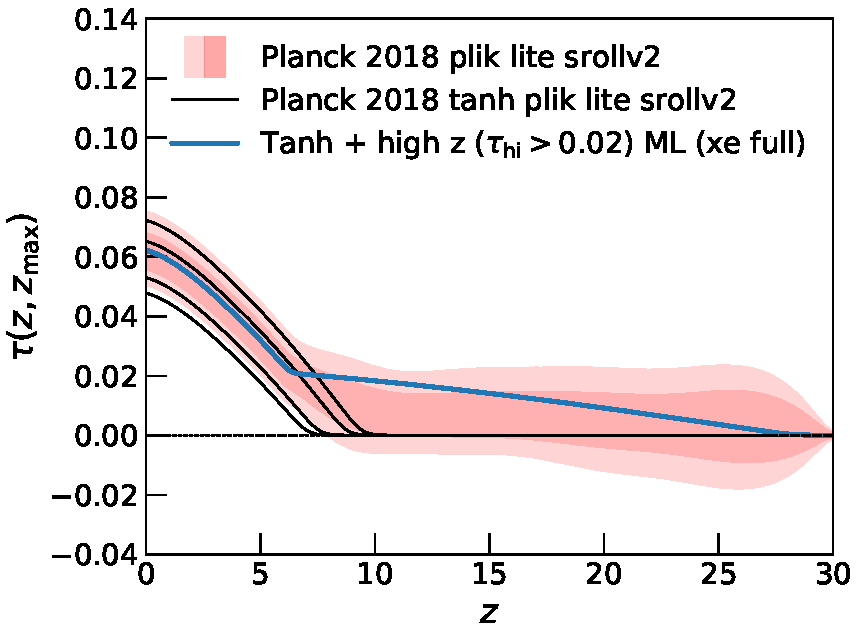
\includegraphics[width=0.450\textwidth]{plots/plot_tau_gtz.pdf}
%\caption{Same as \reffig{plot_taugtz_PC_vs_tanh}, but superimposed with the cumulative optical depth $\tau(z, \zmax)$ of the best-fit two-step model. The two-step model is a toy model that adds a high-$z$ ionization plateau to the standard tanh model with one additional parameter. Compared to the cumulative $\tau$ distributions from PCs, the best-fit two-step model is within the 95\% upper limit of the cumulative $\tau$ constraints at all redshifts. 
%}
%\label{fig:plot_taugtz_two_step_best_fit}
%\end{figure}


%\begin{figure}
%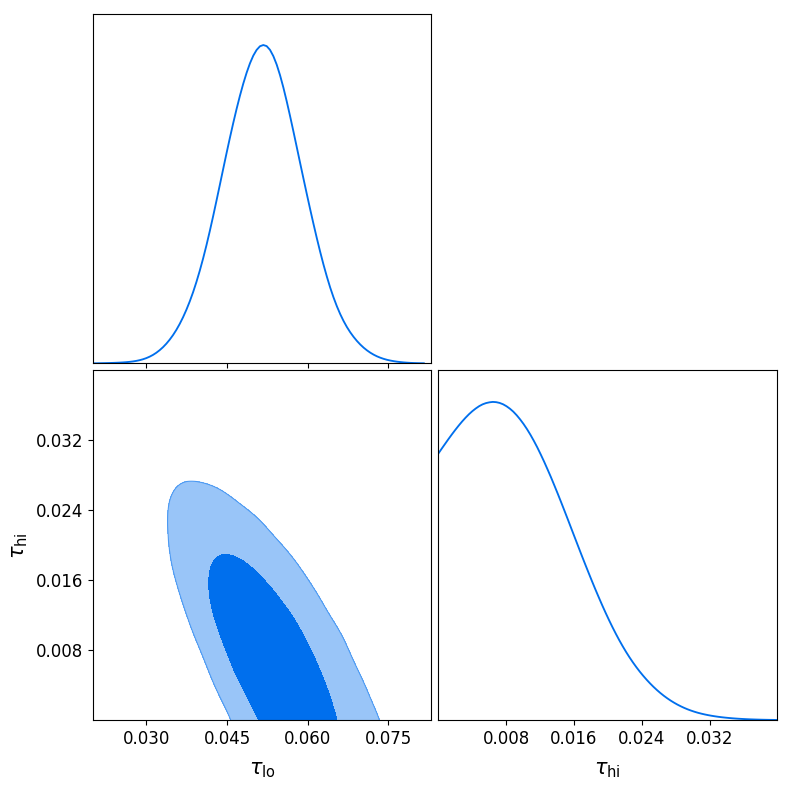
\includegraphics[\textwidth]{results/direct_mcmc/two_parameter_model/tauhi_taulo_chains/pl18_tanh_highz_test2_run1_tri.png}
%\caption{Direct MCMC chains of the two-parameter model with \tauhi and \taulo: triangle plot of \tauhi and \taulo. The marginalized 1D constraints are \taulo = $0.0516 \pm 0.0076$, \tauhi = $0.0100 \pm   0.0066$. The ML model is \taulo = 0.0543 and \tauhi = 0.0054 corresponding to $z_{\rm re} = 7.68$ and $x_{e, \mathrm{min}} = 0.021$.
%}
%\label{fig:two_parameter_model_2D_plot}
%\end{figure}


%\begin{figure}
%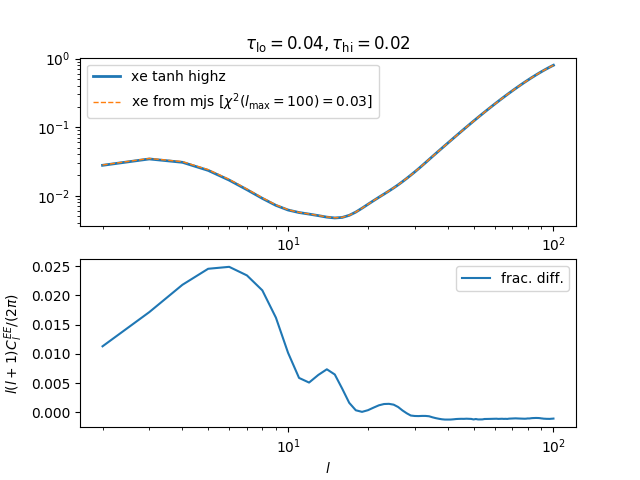
\includegraphics[\textwidth]{results/cosmomc_kde/taulo_prior_test/plot_cls_taulo_0p04_tauhi_0p02.png}
%\caption{Testing \taulo prior -- testing that \taulo $\geq$ 0.04 as \taulo prior is OK, by calculating $\chi^2$ between $C_l$ from full $x_e(z)$ vs PC decomposition of the model (\taulo, \tauhi) = (0.04, 0.02). 
%The $\chi^2 = \sum_{2}^{l_{\rm max}} (\Delta C_l^{EE})^2 / \mathrm{Cov}_l = 0.03$ where $\mathrm{Cov}_l = 2 (C_l^{EE})^2/(2l+1)$. } 
%\label{fig:taulo_prior_test_cl}
%\end{figure}

\section{Model-Independent Results for Optical Depth}

\wh{
While the PC approach to constraining reionization should mainly be used for 
testing wide classes of models efficiently and with their own physically motivated priors, it can also be employed to extract model-independent constraints on the total and cumulative optical depth.  As discussed in \S \ref{sec:cumulative}, since the PC amplitudes are not intrinisically required
to produce physically sensible ionization histories where $0 \le x_e(z) \le x_e^{\rm max}$, this requires imposing physicality priors using Eq.~\ref{eq:individualprior}.  In addition these flat range-bound priors on the PC amplitudes $m_a$, imply implicit priors on the optical depth.   
Finally our fiducial analysis has an explicit prior that reionization occured
at $z<z_{\rm max}=30$.   In this section we present these model-independent results and discuss their robustness to these explicit and implicit priors.
}



%So far no priors on the PC chains have been used. In constructing the kernel density estimate of Section~\ref{sec:effective_likelihood} we used PC chains without priors; and when using the effective likelihood for model testing, it would always be restricted to a particular set of physical models like in the two examples we showed above. To derive model-independent constraints in this section, however, we will now impose the physicality priors of Eq.~\ref{eq:individualprior}. 

%Before we show the cumulative optical depth constraints from PCs, let us first make a note about the impact of the physicality prior chosen for this analysis and clarify some wrong claims against it in the literature.

\subsection{Total optical depth}
\label{sec:note_on_priors}


Using Eqs.~(\ref{eq:mmutoxe}) and (\ref{eq:cumtau}), we can derive constraints on the total optical
depth $\tau=\tau(0,z_{\rm max})$ with the physicality priors of Eq.~\ref{eq:individualprior}.  These are shown in Fig.~XX 

\wh{figure could include $\tau_{\rm PC}$, tanh tau and 2 step}
and correspond to
\beq
\tau_{\rm PC} = 0.0619^{+0.0056}_{-0.0068} \;\; (\texttt{srollv2}),
\label{eq:tau_pc_zmax30}
\eeq  
Notice that the PC mean, while still compatible with the tanh 
tau derived constraints, is almost $0.5\sigma$ higher...


The difference between these results come down to implicit and explicit priors.   Results based on the tanh model requires that reionization happens suddenly at $z_{\rm re}$ and is maintained thereafter.   Therefore, the model has a strong implicit prior that a given a total optical depth $\tau$ comes from $z\lesssim z_{\rm re}$ regardless of whether the data allow or prefer
ionization at higher $z$.  While this prior may be well motivated
theoretically \cite{XX} (sims that give prompt reionization), it should be distinguished from constraints that are data driven.  
This was especially apparent with the Planck 2015 data where
the PC constraints gave $\tau=XX\pm YY$ which differed substantially from the tanh $\tau=XX\pm YY$.  As we shall discuss
below, these differences were even more striking in the implications for the cumulative $\tau$ at high redshift.

PC constraints on the total optical depth do not suffer from assuming a specific class of ionization histories as they parameterize any $x_e(z)$ from $z_{\rm min}=6$ to $z_{\rm max}=30$.
They do of course come with their own priors namely the flat
range-bound ones from Eq.~\eqref{eq:individualprior}.
These have in fact caused some confusion in the literature when interpreted in terms of the total optical depth \cite{Millea:2018bko}.  Here we first review the impact of flatness in PC space as discussed extensively in Ref.~\cite{Heinrich:2018btc} and then highlight the more important role of physicality priors with Planck 2018 data as compared with
2015 data.

 We first note that by virtue of Eq.~\ref{eq:mmutoxe}, the total optical depth receives contribution from all PCs
\beq
\tau_{\rm PC} = \tau_{\rm fid} + \sum_a m_a \tau_a,
\eeq
where $\tau_a$ is the contribution from a unit amplitude PC and $\tau_{\rm fid}$, that from the fiducial model.
The PCs are rank ordered by their expected constraining power and so most of the information on the total optical depth comes from
the first two components
\beq
\tau_{12} = \tau_{\rm fid} + m_1 \tau_1 + m_2 \tau_2 \approx \tau.
\eeq
\wh{possibly redefine
\beq
\tau_{12} =  m_1 \tau_1 + m_2 \tau_2 +
\left(\sum_{a=3}^5 \bar m_a \tau_a + \tau_{\rm fid}\right) \approx \tau.
\eeq
where the term in parentheses is a fixed quantity (refer to eqns/table where tau's and mbars are defined) whose purpose is to remove offsets due to the arbitrary choice of fiducial model.
}
%
% Therefore, while retaining all physical models, they also includes some unphysical models. The authors of Ref.~\cite{Millea:2018bko} (hereafter MB18) raised a concern that these PC priors implies a non-flat prior in $\tau$ and claimed that it biases the PC result of  Ref.~\cite{Heinrich:2016ojb} and accounts for most of the shift between the tanh and PC $\tau$ posteriors. In Ref.~\cite{Heinrich:2018btc}, we showed that the use of our physicality prior does not cause bias for data that is constraining, which includes the Planck 2015 dataset. On the other hand, we showed in Ref.~\cite{Heinrich:2016ojb} that if one adopts the method proposed in Ref.~\cite{Millea:2018bko}. in an attempt to flatten the $\tau$ prior (by multiplying its inverse at each point in the multidimensional PC space), one would actually end up with a biased $\tau$ constraint for the Planck 2015 data. 
%
%We briefly recap the argument below. Let us use $\tau \approx \tau_{12}$ in order to illustrate the impacts of the priors more easily. We first note that by virtue of Eq.~\ref{eq:mmutoxe}, the total optical depth receives contribution from all PCs
%\beq
%\tau = \tau_{\rm fid} + \sum_a m_a \tau_a,
%\eeq
%where $\tau_a$ is the contribution from a unit amplitude PC and $\tau_{\rm fid}$, that from the fiducial model. Because most of the contributions to $\tau$ comes from the first two components (see also Fig. 7 of Ref.~\cite{Heinrich:2018btc} in the Appendix), we can approximate it as
%\beq
%\tau_{12} = \tau_{\rm fid} + m_1 \tau_1 + m_2 \tau_2 \approx \tau.
%\eeq
Due to this linearity, flat priors in $m_1$ and $m_2$ correspond to
flat priors in $\tau_{12}$ for any linear trajectory through the space.   For example, the tanh model trajectory is shown in Fig.~{\ref{fig:plot_mjs_2018_vs_2015}.   Even without the explicit 
construction of a flat tanh $\tau$ prior in \S \ref{sec:example1}, 
the implicit prior from $m_1,m_2$ is already nearly flat. \ch{CH: need to ask a question about this.}

Ref.~\cite{Millea:2018bko} raised a potential objection regarding more general models.  As illustrated in Fig.~\ref{fig:prior_box}, lines of constant $\tau_{12}$ are rotated compared with the $m_1$,
$m_2$ axis.  Therefore, the range-bound flat prior in $m_1,m_2$ (blue square) considered {\it alone} corresponds to a prior that is not flat in $\tau_{12}$ due to the extent  of the allowed parameter space
for each of its values, e.g. at  left corners (Fig.~\ref{fig:prior_box} solid square or lowest $m_1$) of the range $\tau_{12}=0.023$
than at $\tau_{12} = 0.130$ and the implied prior increases linearly from zero between the two.
   Ref.~\cite{Millea:2018bko} suggest 
inverting this prior point-by-point in the $m_a$ parameter space by dividing by the implied prior $P(\tau_{\rm PC}) [ \approx P(\tau_{12})]$ and this reweighting was implemented in the \ch{Planck 2018 paper on cosmological parameters~\cite{Aghanim:2018eyx}}.
First notice that this inversion would in fact then produce a non-flat prior on $\tau$ for the tanh model
that disfavors high values.   This is because
the additional parameter space allowed by the range-bound $m_a$ prior is excluded by the functional form of the model even though the reweighting occurs globally and includes the tanh trajectory as well. 

More generally, to the extent that the data constrain $m_1$ and $m_2$ better than the flat range-bound priors, these priors become irrelevant and the reweighting of Ref.~\cite{Millea:2018bko} becomes erroneously motivated.   To see this, consider a range-bound prior that is rotated to be oriented along constant $\tau_{12}$ (see Fig.~\ref{fig:prior_box}, blue dashed rectangle). \ch{This rotated prior in $m_1-m_2$ space corresponds to a flat prior in $\tau_{12}$ space.}
Had the original prior (blue square) been shifted to slightly lower
$m_1$ and encompassed all of the 95\% CL allowed
region the two priors would yield  identical constraints at the
95\% CL.   This is in spite of the fact that reweighting by $1/P(\tau_{12})$ would still change the original prior but not the
rotated one.  \ch{CH: will try rephrasing.}

The real impact of our range-bound $m_1,m_2$ priors comes from the fact that with the Planck 2018 data, the physicality prior on $m_1$
removes nearly half of the space that would otherwise be allowed by the
data at 95\% CL.  This is in contrast to the Planck 2015 data where only a very small region is removed (see Fig.~\ref{fig:plot_m1m2_2015_vs_2018}).  \wh{Maybe add to the $\tau$ vs $\tau_{12}$ figure a version that does not have this $\tau_{12}$ cut.  Mention that even in the direct tanh constraints, the impact of taking $z\gtrsim 6$ also has the effect of removing some of the low $\tau$ region.}

\wh{But it looks like from our conversation (3/12) that this is a small effect on tanh tau with srollv2.  So instead discuss the impact of our priors - mostly it seems to remove negative tau contributions at high $z$ (from looking at the internal Fig 11) and the shifts relative to tanh tau are mostly just the ability to add a small amount of high z ionization that tanh excludes by its form.  Rework this discussion below but I think it is compatible with our conclusion that that our conservative inclusion of some unphysical cases is not biasing our model independent results and instead it is the tanh model that carries a small bias due to its assumed form that excludes the small amount of high-z ionization that is still allowed by the data.}.

As discussed in \S \ref{sec:cumulative}, our range-bound priors 
are conservative in the sense that all the cases that are excluded are definitely unphysical but some of the cases that are included
may also be unphysical since their physicality depends on higher order PC components that are explicitly truncated in the analysis.  On the other hand the tanh model provides an explicitly physical example whose trajectory runs close  and nearly parallel to the our physicality prior in the allowed region and so we do not expect the bias incurred by 
including these possibly \wh{unphysical cases} to be large. 
%\ch{CH: sorry, what do we mean by these models here?}  
In any case, using PCs to 
test explicitly physical models as in \S \ref{sec:example1} and
\ref{sec:example2} cannot be affected by our conservative physicality
cut.

Finally, we check that our results (Eq.~\ref{eq:tau_pc_zmax30}) are robust to
 extending the PC
range to
$z_{\rm max}=50$ which is negligibly different
\beq
\tau_{\rm PC,\, \zmax=50} = 0.0626^{+0.0061}_{-0.0072}\;\; (\texttt{srollv2}).
\eeq
Reverting the Planck 2018 likelihood to \texttt{lowE} at $z_{\rm max}=30$ would give
\beq
\tau_{\rm PC} = 0.0582 ^{+0.0072}_{-0.0083}\;\; (\texttt{lowE}).
\eeq
As with the tanh model, the \texttt{srollv2} likelihood provides tighter constraints that shift the distribution toward higher optical depth.










%models that 
%In Fig.~\ref{fig:prior_box}, we show the Planck 2018 constraints (ellipse) in the $m_1-m_2$ plane along with constant lines of $\tau_{12}$ (light gray). The solid blue box corresponds to the physicality prior, whereas the dashed blue box is constructed to be aligned with the directions of the constant $\tau_{12}$ lines, so that when projected onto the $\tau_{12}$ directions, gives a true flat $\tau_{12}$ prior. The physicality prior upon projection would correspond to a linearly rising prior in $\tau_{12}$ over the region where the posterior has support. One would be eager to conclude that this produces a biased constraint on $\tau_{12}$. However, because the Planck data is more constraining than the prior in $m_1$ and $m_2$, (the ellipse occupying a much smaller area in one part of the prior box), the value of the prior at high $\tau_{12}$ becomes irrelevant for the posterior. However, if one tries to mitigate for the $\tau_{12}$ prior by multiplying the inverse prior value at each point in the PC space over the area where data is more constraining than the prior, then one would bias the posterior toward lower $\tau_{12}$ in this case. 

%What is then the true impact of this physicality prior we have imposed. We have established that the orientation of the prior box in the $m_1-m_2$ plane does not matter for this dataset since the data is more constraining than prior. However, the location of the data constraint does matter, as the prior box currently cuts off half of the ellipse in the Planck 2018 data (a larger amount than in Planck 2015). The consequence of this cut in the $\tau$ constraints essentially amounts to excluding models not fully ionized models by $\zre \sim 6$, as consistent with observational constraints. 

%The other impact of using the physicality prior is that some unphysical models are included inside the prior. We reiterate that we do not adopt this prior for the KDE and unphysical models do not impact results when actually testing physical models using the effective likelihood code. We will show in the next section that their impact on the model-independent $\tau$ results are also minimal.  

%[add a sentence to reiterate that the shift between PC and steplike model seen in the Planck 2015 is not due to the use of physicality prior? and some other Marius/Planck paper points?]

%[restore some text about evolution of planck data and HFI systematics causing PC-tanh shifts in Planck 2015 data? And address the claim: ``In the Planck 2018 paper on cosmological parameters, the reduction of optical depth from the PC results seen in the Planck 2018 data compared to the Planck 2015 data was attributed to the reduction of HFI systematics, with subdominant contribution from prior."] 
%They also proposed a method to flatten the $\tau$ prior by multiplying its inverse at each point in the multidimensional PC space. The authors claim that adopting the physicality priors in Ref.~\cite{Heinrich:2016ojb} contributed to a large fraction of the shift in the $\tau$ posterior between the tanh and the PC results in the Planck 2015 data. 

 \begin{figure}
          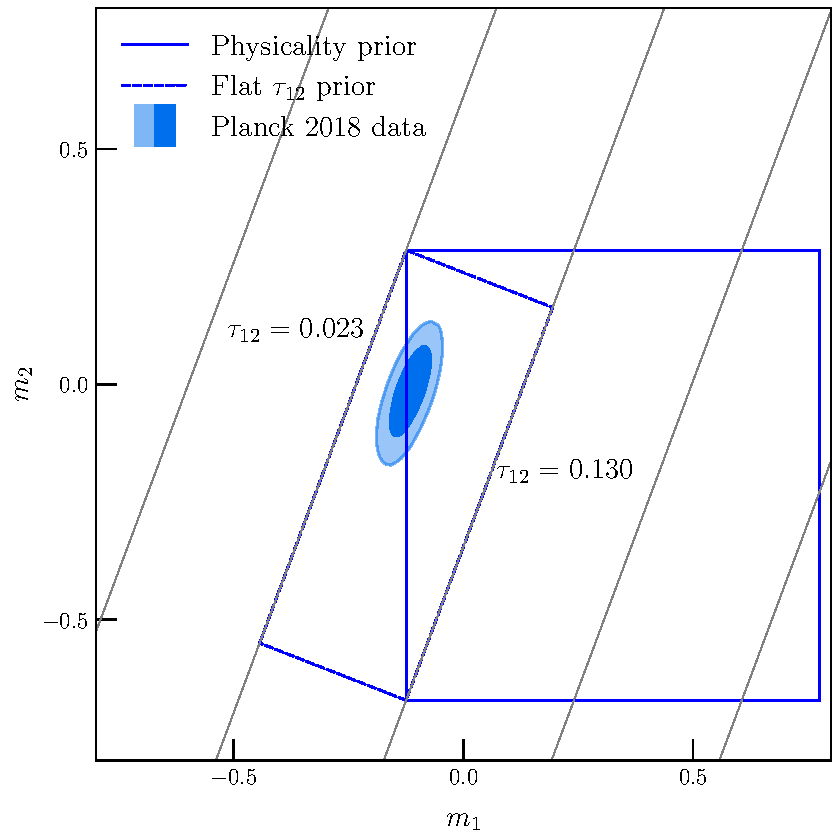
\includegraphics[width=0.9\columnwidth]{paper/plots/pl18_pc_zmax30_pliklite_srollv2_1015_plot_rotated_box_flat_tau12.pdf}
          \caption {Priors on the $m_1-m_2$ parameter space: the physicality prior (inset square, solid lines) and a flat prior in
           $\tau_{12}$ and in $m_1-m_2$ (rotated rectangle, dashed lines) 
           %\ch{CH: [why is this flat in m1 and m2?]} 
           % flat in 2D or locally flat
           which are aligned with lines of constant $\tau_{12}$ (light gray lines). Note that although the physicality prior allows for more parameter space at higher $\tau_{12}$, that is also the region excluded by the data constraints (ellipses). The only difference in the allowed region is that the physicality prior clips the low $m_1$ portion of the allowed region due to the physicality condition and the assumption that reionization occurs at $z\ge 6$. \ch{CH: numbers changed according to new definition with mean of m3, m4, m5 obtained from chains with priors (shifted numbers by about 0.005 in tau.} \ch{CH: this plot is done}} 
          \label{fig:prior_box}
\end{figure}

\begin{figure}[ht]
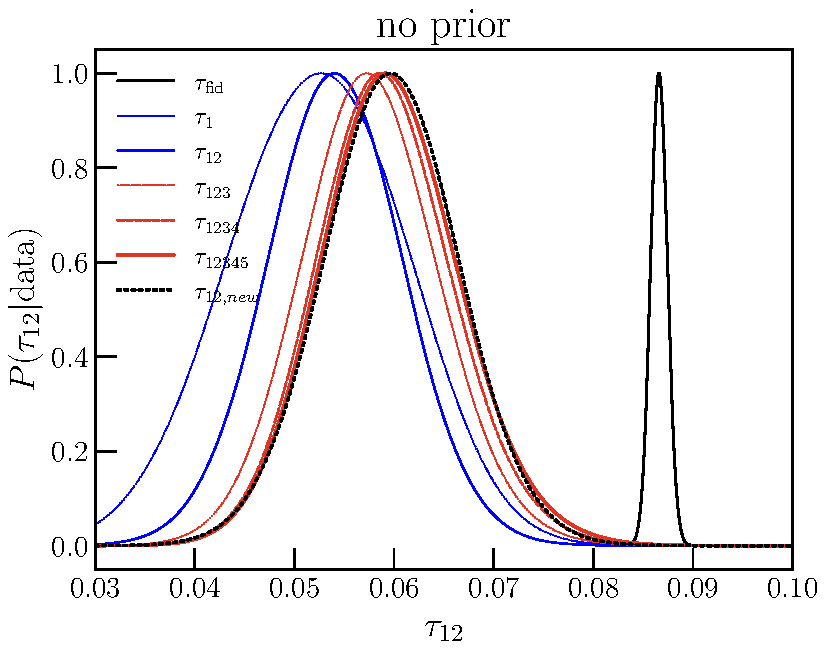
\includegraphics[width=0.48\textwidth]{results/tau_pc_decomposition/plot_taumj_decomposition_apply_cut_False_pl18_pc_zmax30_pliklite_srollv2_1015.pdf}
\caption{$\tau_{12,new}$ - \wh{this is an internal plot - leave in for now but also make a version for the paper: just $\tau_{12}$ vs $\tau_{\rm PC}$ in our new convention with and without prior either as a single or separate panel whichever is clearer.}}
\label{fig:tau12}
\end{figure}

\begin{figure}[ht]
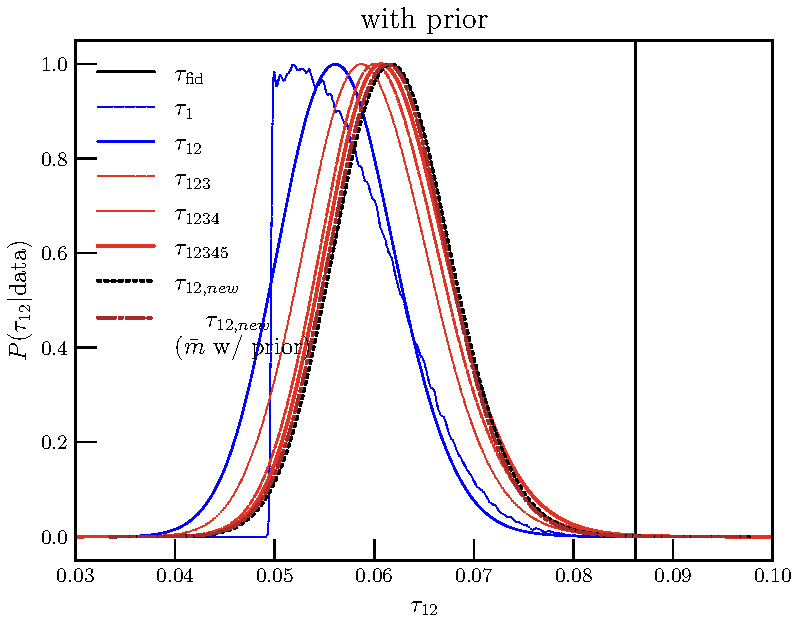
\includegraphics[width=0.48\textwidth]{results/tau_pc_decomposition/plot_taumj_decomposition_apply_cut_True_pl18_pc_zmax30_pliklite_srollv2_1015.pdf}
\caption{ \ch{CH: this is the same as above but with priors; also tested that $\tau_{12, new}$ with mean of m3, m4, m5 computed from chains with prior applied performs better here (as expected) from chains without prior.}}
\label{fig:tau12}
\end{figure}

\begin{figure}[ht]
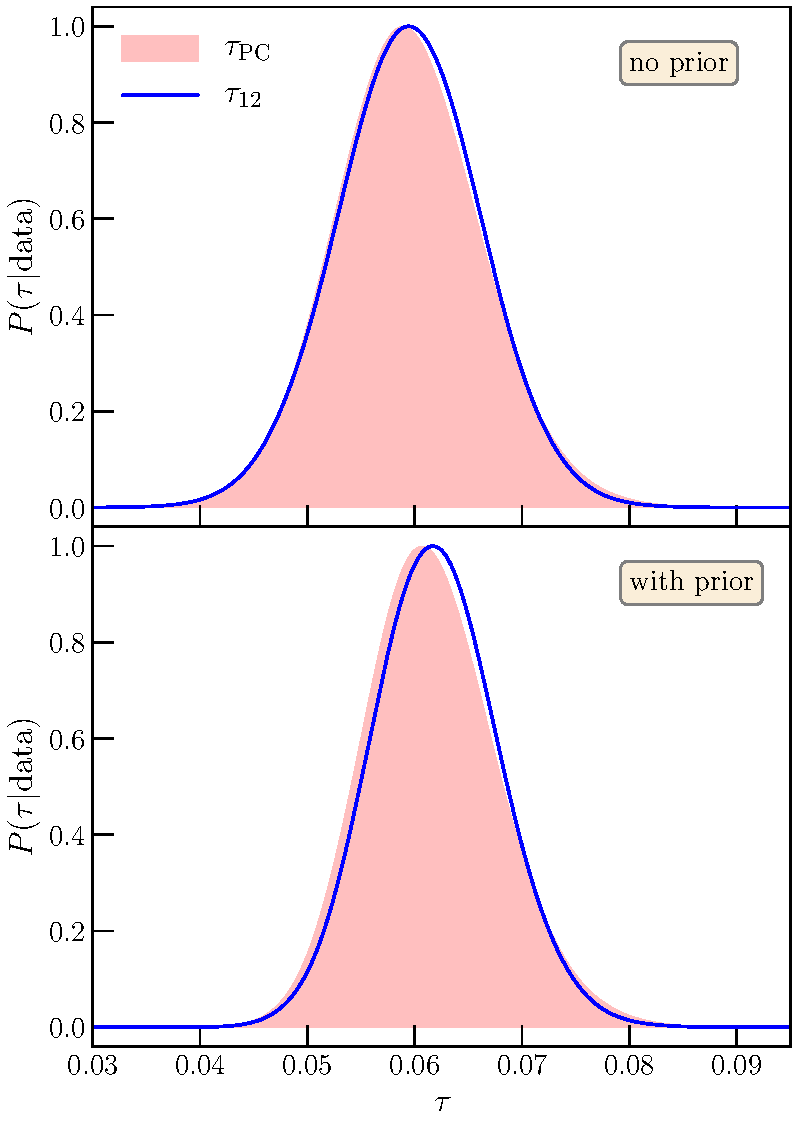
\includegraphics[width=0.48\textwidth]{paper/plots/plot_tau12_new_apply_cut_False_vs_True_pl18_pc_zmax30_pliklite_srollv2_1015_two_panels.pdf}
\caption{$\tau_{12}$ \ch{(CH: Official version used for paper; plot is done.\\
More details: took out the cosmology part, only shrunk posteriors very slightly and shifted them a bit to the left for the top panel; with prior version now added in the bottom panel, it uses the mean from m3, m4, m5 that are computed from the chains with prior as well.)}}
\label{fig:tau12}
\end{figure}

\begin{figure}[ht]
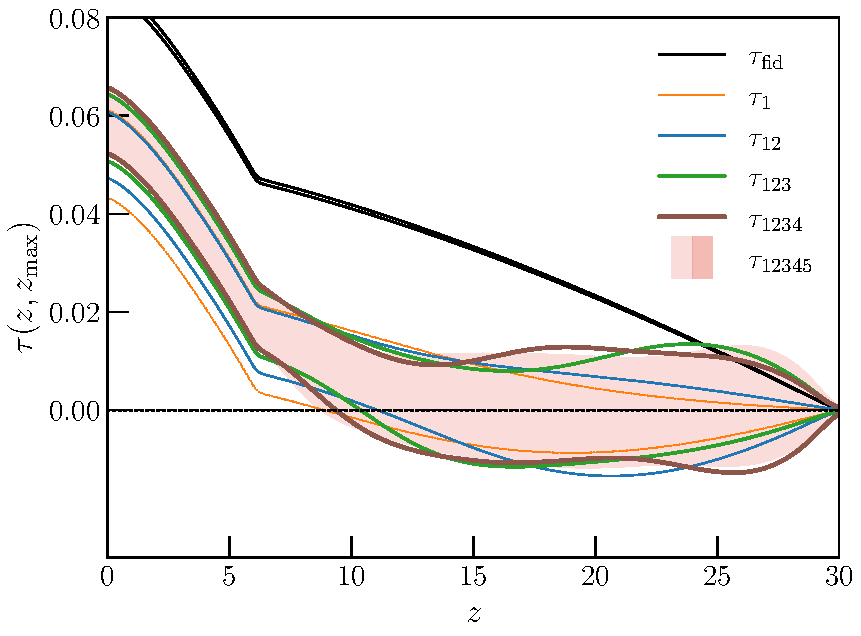
\includegraphics[width=0.48\textwidth]{results/tau_pc_decomposition/pl18_taugtz_pc_decomposition_68_only.pdf}
\caption{$\tau$ decomposition (68\% C.L. only) \wh{this is a temporary plot for internal purposes - what I'm seeing here is that without the physicality cut the high $z$ side goes unphysically negative.  I think this is consistent with our description and the $S_1$ curve.}}
\label{fig:tau12}
\end{figure}

\begin{figure}[ht]
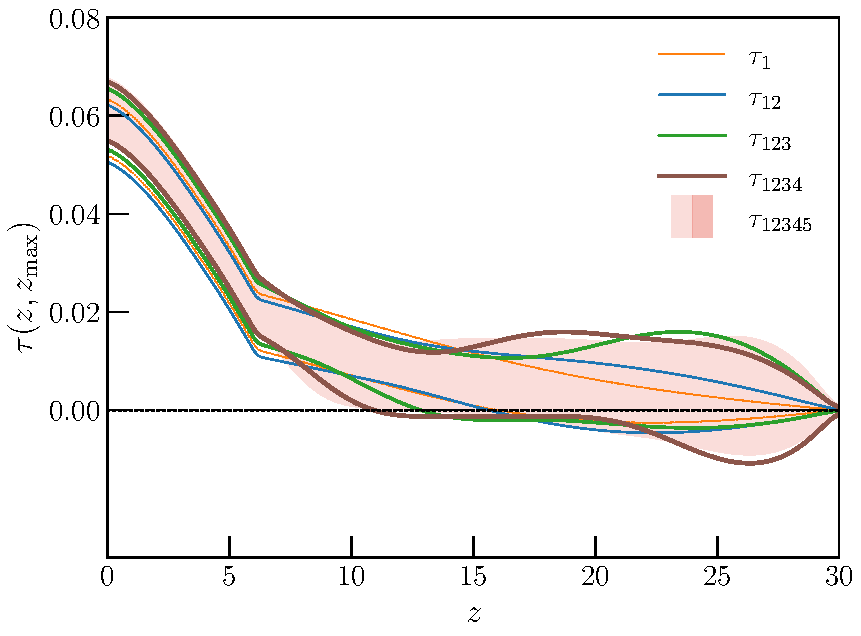
\includegraphics[width=0.48\textwidth]{results/tau_pc_decomposition/pl18_taugtz_pc_decomposition_68_only_apply_cut_True.pdf}
}
\caption{\ch{Internal for now (with prior version)}}
\label{fig:tau12}
\end{figure}


%
%
%
\subsection{Cumulative optical depth}

The differences between model dependent and model independent approaches are larger for the allowed cumulative optical depth $\tau(z, \zmax)$ at high $z$
compared to the total optical depth of the previous section.
The main results are again related to the $m_1$ and $m_2$ PC constraints. 
As discussed in Ref.~\cite{Heinrich:2016ojb}, raising $m_1$ increases the  optical depth at all $z$ but with a larger weighting at high $z$ whereas
raising $m_2$ shifts the optical depth from low $z$ to high $z$.  
Consequently, as shown in Fig.~\ref{fig:prior_box}, the second aspect of PC constraints beyond the well constrained total optical depth, is a positive
correlation between the two components that represents the high to low $z$ 
contribution to the total optical depth.  Any finer detail in the ionization history is much more poorly constrained.

\ch{[CH: Fig.~\ref{fig:plot_taugtz_2018_with_vs_without_physicality_prior} needs to go somewhere]}
% with this prior you still have that $\tau(>z)$ plot includes unphysical models (however, most likely total tau doesn't change, and if any bias from unphysical models, it would lower high-z tau).\\

In Fig.~\ref{fig:plot_taugtz_2015_vs_2018_simallEE_vs_2018_srollv2} top panel, we compare the 68\% and 95\% confidence level contours in $\tau(z, \zmax)$ for the Planck 2015 (red regions) and the Planck 2018 results (solid lines) using all 5 PCs.
\wh{remind the reader about impact of PC filtering smoothing out features in redshift - refer to the tanh examples to illustrate}
In the lower panel, we compare the Planck 2018 results for the two different low-$\ell$ $EE$ likelihoods.   Notice first the dramatic improvement in the
constraint at high-$z$.  Whereas the Planck 2015 allowed and even preferred
finite optical depth at $z\gtrsim 15$, Planck 2018 no longer does....
On the other hand, some optical depth is still allowed 
\beq
\tau_{\rm PC}(15, 30) < 0.023 \; (95\%\; \mathrm{C.L.})\;\;(\texttt{srollv2}),
\eeq
in contrast with the tanh model where it is strictly forbidden in the direct analysis and in the PC filtered effective analysis only enters due to the smoothness of the first few PCs in redshift space.
\wh{contrast this with Flexknot and talk about compatibility with example 2.}

We also show using a separate PC chains with $\zmax = 50$ that there is no evidence for optical depth at $z>30$. 
In Fig.~\ref{fig:plot_taugtz_zmax30_vs_zmax50}, we show that the 68\% and 95\% C.L. contours of $\tau(z, \zmax)$ are consistent between the $\zmax = 30$ (red regions) and $\zmax = 50$ results (black lines).

%Furthermore, their total optical depth constraints are practically identical: %
%\beq
%\tau_{\rm PC,\, \zmax=30} = 0.0619^{+0.0056}_{-0.0068}\;\; (\texttt{srollv2}),
%\eeq
%and
%\beq
%\tau_{\rm PC,\, \zmax=50} = 0.0626^{+0.0061}_{-0.0072}\;\; (\texttt{srollv2}).
%\eeq
%
%Compared the \texttt{lowE} likelihood results, 
%\beq
%\tau_{\rm PC,\, \zmax=30} = 0.0582 ^{+0.0072}_{-0.0083}\;\; (\texttt{lowE}),
%\eeq
%and
%\beq
%\tau_{\rm PC,\, \zmax=50} = 0.0582^{+0.0077}_{-0.0088}\;\; (\texttt{lowE}).
%\eeq
%the \texttt{srollv2} error bars on PC $\tau$ was reduced by about 20\%, and the central values rose by about half a sigma. [wanna comment more here?]
%

For the high-redshift optical depth, we also obtain consistent upper limits
%\beq
%\tau_{\rm PC}(15, 30)< 0.023 \; (95\%\; %\mathrm{C.L.})\;\;(\texttt{srollv2}),
%\eeq
%[double check on full chain (from 10/15) this is from 09/30.]
%and 
\beq
\tau_{\rm PC}(15, 50) < 0.022 \; (95\%\; \mathrm{C.L.})\;\;(\texttt{srollv2}).
\eeq

\begin{figure}[ht]
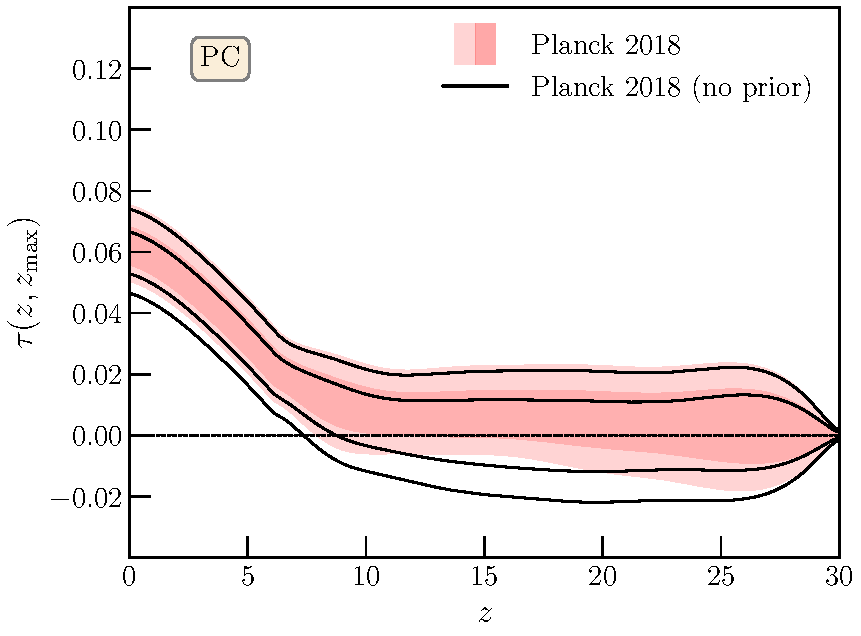
\includegraphics[width=0.48\textwidth]{paper/plots/pl18_taugtz_pc_zmax30_pl18_srollv2_with_and_without_physicality_prior.pdf}
\caption{Comparison of the 68\% and 95\% C.L. constraints on the cumulative optical depth $\tau(z, \zmax)$ from PC chains with (shaded) and without (black) applying the physicality prior. While the lower limits on $\tau(z, \zmax)$ are lowered when more unphysical models are included, the upper limits do not vary significantly (slightly lowered).  The total $\tau$ distribution is broadened only toward the lower $\tau$. \ch{Discuss in text the small difference in upper limits at $\tau(15, \zmax)$ is such that if one could remove unphysical models inside our current prior range, $\tau(15, \zmax)$ upper limit would be only slightly looser.} \ch{CH: plot is done}
}
% no prior: 95\% C.L.  = [-0.01935756790924691, 0.021029019067727237]
% with prior: {'z': 15, 'mean': 0.00694422689213187, 'std': 0.007568921831067864, 'limit68': [-0.0007215571045808687, 0.014684826477572082], 'limit95': [-0.006316156744039184, 0.02284538046347211]}
%
%}
\label{fig:plot_taugtz_2018_with_vs_without_physicality_prior}
\end{figure}


\begin{figure}[ht]
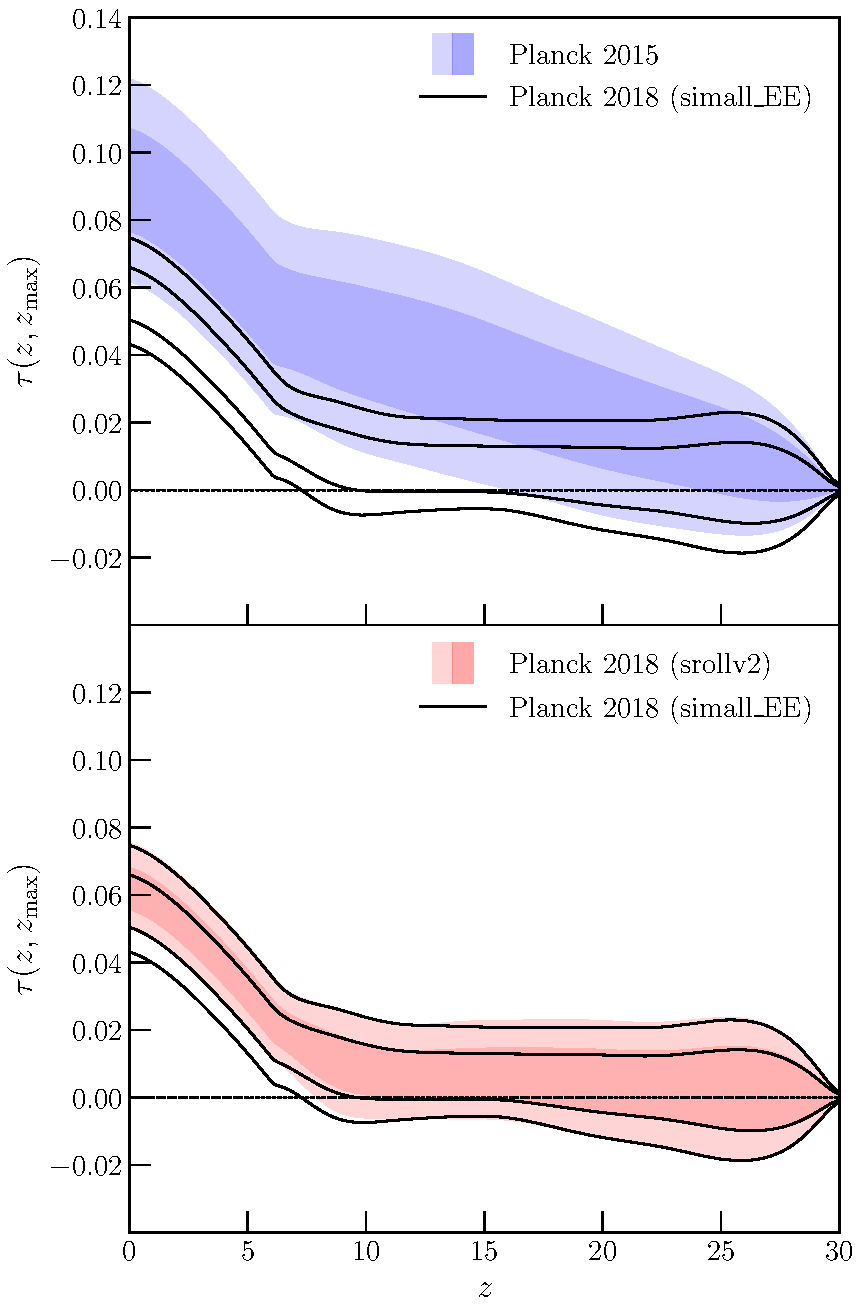
\includegraphics[width=0.45\textwidth]{paper/plots/pl18_taugtz_pc_zmax30_pl15_vs_pl18_simallEE_vs_pl18_srollv2.pdf}
\caption{Comparison of the 68\% and 95\% C.L. constraints on the cumulative optical depth with different Planck likelihoods. \textit{Top}: The Planck 2015 vs Planck 2018 likelihoods, the latter including the official low-$\ell$ $EE$ likelihood $\texttt{simallEE}$. \textit{Bottom}: The Planck 2018 likelihoods using $\texttt{simallEE}$ for the low-$\ell$ $EE$ likelihood vs \texttt{srollv2} which has better foreground cleaning. Both yield consistent high-redshift constraints, whereas the \texttt{srollv2} likelihood tightens the lower limit on the low-$z$ contribution, resulting on a tighter lower limit and higher mean for the total $\tau$. \ch{CH: plot is done}
}
\label{fig:plot_taugtz_2015_vs_2018_simallEE_vs_2018_srollv2}
\end{figure}


\begin{figure}[ht]
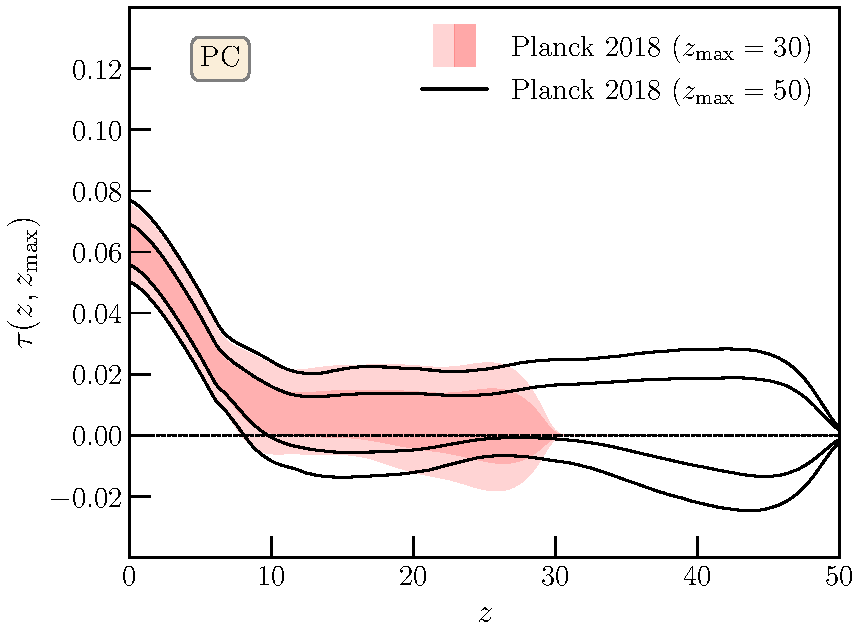
\includegraphics[width=0.48\textwidth]{paper/plots/pl18_taugtz_pl18_srollv2_pc_zmax30_vs_zmax50.pdf}
\caption{Comparison of the 68\% and 95\% C.L. constraints on the cumulative optical depth from PC chains with $\zmax = 30$ vs $\zmax = 50$ using the Planck 2018 likelihoods. The constraints on the cumulative high-redshift optical depth are shown to be robust to $\zmax$. Both the low-redshift constraints and the high-redshift upper limits agree well. \ch{CH: plot is done}
}
\label{fig:plot_taugtz_zmax30_vs_zmax50}
\end{figure}


\section{Conclusion}
\label{sec:conclusion}

In conclusion, we used constraints on reionization principal components with respect to the large-scale $EE$ data to produce a fast and accurate effective likelihood for the final release of Planck 2018 data. In lieu of the official $\texttt{simallEE}$ likelihood for low-$\ell$ $EE$ we used the independent later release of the $\texttt{srollv2}$ likelihood in 2019 which has better foreground cleaning allowing for slightly improved parameter constraints. Our effective likelihood code package is called $\textsc{Relike}$ [to be changed] and is available publicly on Github. This code is beneficial for the community for the purpose of testing \textit{any} global ionization history between $6 < z < 30$ with the Planck data without having to modify CAMB which can be very cumbersome to do. The convergence time to reach the Gilman-Rubin criteria $R_{-1} < 0.01$ is about 300 times less with the Relike code than with a traditional MCMC sampling of the Planck likelihood for the one-parameter canonical tanh model. 

To test this effective Planck likelihood code, we used two examples: 1) a canonical tanh model with a single transition redshift, and 2) a two-parameter model consisting of two tanh transitions allowing in addition for a high-redshift ionization plateau compared to the first example. We demonstrated accuracy of the Relike code for both examples by comparing the constraints on the reionization model parameters with those obtained from directly sampling the full Planck likelihood and using a modified CAMB code. We also showed great agreement between the confidence levels of the cumulative optical depth evolution between the 5-PC representation and the exact ionization model.

Besides conducting explicit model testing with the Relike code, we also obtained model-independent constraints on the reionization history using the PC chains themselves. We summarize these results below.

\begin{itemize}

    \item {We obtained the constraint on the total optical depth $\tau_{\rm PC} = 0.0619^{+0.0056}_{-0.0068}$ (68\% C.L.) 
    using PCs and the Planck 2018 likelihoods using the \texttt{plik\_lite\_TTTEEE+lowl+srollv2} likelihood combination.}
    
    \item {The better foreground cleaned \texttt{srollv2} likelihood allowed to tighten the PC constraint on $\tau$ and shifted it toward slightly higher values when compared with the \texttt{plik\_lite\_TTTEEE+lowl+lowE} result  $\tau_{\rm PC} = 0.0582 ^{+0.0072}_{-0.0083}$ (68\% C.L.).}
    
    \item {We checked the robustness of our $\zmax=30$ results by performing a PC analysis of the Planck data with $\zmax = 50$. The results are changed negligibly: $\tau(15, 50) < 0.022 $ (95\% C.L.) in comparison with $\tau(15, 30) < 0.023$ (95\% C.L.).}
    
     \item {Though our high-redshift optical depth constraints are looser than those from the Planck 2018 cosmological parameter paper $\tau(15, 30) < 0.007$ (95\% C.L.) obtained from another model-independent method called FlexKnot, we have tested using explicitly the tanh high-$z$ toy model (without using any PCs) that an $\tau(15, 30) < 0.02$ (95\% C.L.) [get more precise numbers] is still allowed (see Fig.~\ref{fig:plot_taugtz_two_step_contours}), which is more consistent with our PC results.}
     
\end{itemize}

We clarified some confusion raised in the literature on the effects of applying a range-bound prior on the PC amplitude during the analysis, and demonstrated that these priors, though they include some unphysical ionization models, do not affect the total $\tau$ constraint and the high-redshift optical depth upper limits significantly. In any case, as shown in Fig.~\ref{fig:plot_taugtz_2018_with_vs_without_physicality_prior} removing more unphysical models would only loosen the high-$z$ optical depth upper limit, in contrary to what was claimed in Ref.~\cite{Millea:2018bko}. The shift from a higher to lower total $\tau$ from Planck 2015 to Planck 2018 in any model-independent is however due to the use of XX data as demonstrated by Ref.~\cite{Millea:2018bko}, in relation to better systematics reduction on the low multipoles $l<10$ [check number]~\cite{Heinrich:2018btc}. [cite also a Planck paper].

\begin{itemize}
    \item other interesting points to discuss and add 
    \item future outlook (mention joint analyses)
\end{itemize}

\bibliography{rei.bib}

\appendix



\subsection{Comparison to previous results}
\wh{integrate this into the model sections}

The Planck collaboration has released constraints on the total optical depth $\tau$ with a steplike model parameterized by the tanh function, which has evolved from $\tau = 0.067 \pm 0.022$ (Planck 2015) to $\tau = 0.055 \pm 0.009$ (Planck 2016), then to $\tau = 0.0506 \pm 0.0086$ (Planck 2018) [cite papers]. The major improvement comes from clean-up of systematics in the High Frequency Instrument (HFI) data. 

In Planck 2018 VI, using only lowE data and fixing all cosmological parameters including $A_s e^{-2\tau}$, the optical depth constraints was found to be $\tau = 0.0519^{+0.0030}_{-0.0079}$ for the tanh model, 
$\tau = 0.0504^{+0.0050}_{-0.0079}$ 
for the FlexKnot method (with flat $\tau$ prior) and 
$\tau = 0.0487^{+0.0038}_{-0.0081}$
for the PC method but using the prior inversion procedure
discussed Section~\ref{sec:note_on_priors} and attributed to the slightly lower central value from the PC method to the fact that the priors contain unphysical models. [do we want to check whether the prior inversion procedure could cause a shift at this level? do we want to evaluate this statement?]

They also found the upper limit on high-redshift optical depth to be: $\tau(15, 30) < 0.006$ for the FlexKnot method with a flat $\tau(15, 30)$ prior or $<0.007$ with a flat knot prior. The PC result for the upper limit was not computed. 

Compared to our PC results ($\tau(15, \zmax)_{\rm PC,\, \zmax=30} < 0.023 \; (95\% \mathrm{CL})$), the FlexKnot upper limits are too stringent. The difference is not attributed to the inclusion of unphysical models due to the truncation at 5 PCs as we showed in Section~\ref{sec:example2} with a concrete example of the two-step model. We showed that for this chosen physical model, the $\tau(15, 30)$ upper limits derived from the full Planck likelihood without using any PCs were already not compatible with the FlexKnot upper limits, while the PC results were compatible. So the discrepancy cannot be attributed to the prior choice in the PC results. It also seems that the inclusion of unphysical model would in any case shift the optical depth at high-redshift toward more negative values, which would decrease rather than increase the upper limit. 

[just noticed that our tau(15, 30) $<$ 0.023 result is with srollv2, and flexknot tau(15,30) $<$ 0.007 is with lowE likelihood. In our analysis lowE to sroll2 had a 0.004 increase in total tau. I should run the tau(15, 30) constraint on the lowE chain as well just to double check.]

[Need to address Planck2018 cosmology paper claim: ``The PCA result is slightly lower, and is partly affected by the imperfect physicality priors that allow unphysical negative ionization fractions."]

[Also, they only used lowE likelihood, fixed all other cosmological parameters (including $A_s e^{-2\tau}$). Wondering if that does anything to the difference between our results]

%%%%%%%%%%%%%%%%%%%%%%%%%%%%%%%%%%%%%%%%%%%%


\section{Outline (in progress)}

\begin{enumerate}
    \item{Intro}
        \begin{enumerate}
            \item 1st paragraph: CMB, reionization, why important
            \item discuss modeling of ionization history in CMB inference, tanh vs PCs (fail to capture high-z; PC captures complete parameter space), mention flex knots/other methods; cite previous PC works.
            \item give context about Planck final results; latest srollv2 likelihood, important to harness all information available, PC allows us to do that and turn into an effective likelihood.
            \item this is what we did: we obtain PC results for Planck 2018, and turn PC chains into a effective likelihood for ionization history: highlight key points like fast inference, entire model space up to zmax 30, code publicly available.
            \item we also compared to Planck official results, which is over stringent at high z, which gives additional motivations for using this likelihood; verified no hint of ionization at z>30; state any additional results.
            \item break down of sections.
        \end{enumerate}

	\item{Background}
		\begin{itemize}
			\item{Reionization Principal Components}	
			\item{Kernel Density Estimate}
		\end{itemize}
	\item{Planck 2018 PC results:\\
		- can discuss discrepancy here on high-redshift tau($>$15) constraints.\\
		- compare with our own 2015 PC results
		- zmax = 30 vs 50}
	\item{Effective Likelihood}
		\begin{itemize}
			\item{Code Description}
			\item{Examples - one and two parameter models}
		\end{itemize}
	\item{Discussion}
		
\end{enumerate}

------ \textbf{Some Numbers} ------ \\

\textbf{Planck official results 2015, 2016, 2018} \\

\begin{itemize}
    
    \item Planck 2015 results (LFI): $\tau = 0.067 \pm 0.022$ (68\%) \\

    \item Planck 2016  intermediate results (LFI): $\tau = 0.055 \pm 0.009$ (68\%) \\
    
    \item Planck 2018 results: $\tau = 0.0506 \pm 0.0086$ (68\%) \\

\end{itemize}

\textbf{Planck 2018 paper} \\

Here lowE means lowE data only, fixing all other cosmological parameters including $A_s e^{-2\tau}$\\

\begin{itemize}

\item $\tau = 0.0519+0.0030-0.0079$ (lowE; flat $\tau$ prior; TANH)(68\%); \\

\item $\tau = 0.0504+0.0050
-0.0079$ (lowE; flat $\tau$ prior; FlexKnot)(68\%); \\

\item $\tau = 0.0487+0.0038
-0.0081$ (lowE; flat $\tau$ prior; PCA)(68\%).

\end{itemize}

\textbf{Upper limit on high-redshift optical depth} (only given for the FlexKnot method):

$\tau(15, 30) < 0.006$ (lowE, flat $\tau(15, 30)$, FlexKnot); \\

$\tau(15, 30) < 0.007$ (lowE, flat knot, FlexKnot).\\

Statements to address:

\begin{enumerate}
    \item {\textbf{Statement on prior in Planck 2018}:  ``Heinrich \& Hu (2018) construct a prior that is uniform on $\tau$, but which increases the allowed unphysical parameter space and is chosen a posteriori. Here we instead use the flat prior constructed by the procedure described in Millea \& Bouchet (2018) and Handley \& Millea (2019), which does not admit extra unphysical models and gives the most generic prior that leaves the prior on $\tau$ uniform."}
    
    \item {Is this statement on tanh in Planck 2018 paper correct?} ``The TANH result gives slightly higher optical depth than the others, which is primarily driven by the fixed duration of reionization assumed." \\
    
    \item{\textbf{Other comments on our PC prior giving higher optical depth}: ``The PCA result is slightly lower, and is partly affected by the imperfect physicality priors that allow unphysical negative ionization fractions." and ``Millea \& Bouchet showed that the majority of this (2$\sigma$) preference disappeared when using the lower-noise Planck HFI SimLow likelihood (intermediate results reduction of systematics), with an additional sub-dominant effect due to the choice of prior."}
    
\end{enumerate}

How likelihoods and systematics evolved over time:

\begin{enumerate}
    \item 
    \item {Planck 2018 paper attribute the 2018 upper limit on $\tau(15, 30)$ being \textbf{about 3 times more} stringent than the intermediate results by Millea \& Bouchet to the $SimLow \rightarrow SimAll$ where there was better control of systematics in HFI polarization.}
\end{enumerate}


[high redshift going away should be attributed to better control of systematics in HFI polarization data (changes in the SimAll likelihood compared to SimLow) [cite Planck 2018 results cp]]

\end{document}


% Notes:
% tau1 = (taulo + tauhi) --> (zre, xemin) --> xe(z) ==> tau2 ==> mjs --> tau3(mjs)
% taulo + tauhi = tau_desired 